\documentclass{article}

% The amssymb package provides various useful mathematical symbols
\usepackage{amssymb}
\usepackage{graphicx}
\usepackage[a4paper,margin=1.2in]{geometry}

\begin{document}

\title{DeerAnalysis2018 User Manual}

\author{G. Jeschke \\ ETH Z\"urich \\ Wolfgang-Pauli-Str. 10, 8093 Z\"urich, Switzerland \\ Gunnar.Jeschke@phys.chem.ethz.ch \\ http://www.epr.ethz.ch/software/index}

\maketitle 

% main text
\section{Purpose of the program}
\label{purpose}

The program DeerAnalysis2018 can extract distance distributions from dead-time free pulse ELDOR data (constant-time and variable-time four-pulse DEER) \cite{pannier2000,jeschke2004b}. Furthermore, it can be used for direct comparison of primary data of similar samples \cite{jeschke2004a}. With some caution \cite{jeschke2001} the program may also be applied to the analysis of dead-time free double-quantum coherence EPR experiments \cite{borbat1999}. It should not be used for data from experiments that have a significant dead time,
%
\begin{equation}
	t_{d}> 2 r^{3} \mathrm{ns} \ \mathrm{nm}^{-3} ,
\end{equation}
where $r$ is the shortest distance in the distribution.

Except for fits of two user-defined models for three-spin systems \ref{fit_existing}, the program assumes isolated spin pairs. If more than two spins are coupled (e.g. spin-labeled protein oligomers), distance distributions are only approximate with artifact contributions at both short and long distances \cite{jeschke2009}. DeerAnalysis2018 allows for an approximate correction of these contributions by the 'ghost suppression' feature.

The statistics information provided by earlier versions of DeerAnalysis if the statistics toolbox was available, is not longer provided due to a change in the used Tikhonov regularization routine.

The underlying mathematical problem is (moderately) ill-posed, i.e., quality of the analyzed data is very crucial. Pre-processing tools are implemented to correct for experimental imperfections (phase errors, displacements of the time origin of the modulation) and to separate the intramolecular distances of interest from the intermolecular background contribution. Furthermore, the program provides several independent approaches for extracting the distance distribution, which helps to get a feeling for the reliability of the distribution. Characterization of the distance distribution in terms of its mean value $\left\langle r \right\rangle$ and width (standard deviation $\sigma_{r}$) is usually reliable \cite{jeschke2004a} and is therefore a standard output. The performance of the different approaches for data analysis depends on the type of distance distribution (narrow or broad peaks or both) and was discussed in some detail in Ref. \cite{jeschke2004a}.

DeerAnalysis2018 features a module for validation of distance distributions obtained by Tikhonov regularization. With this module a systematic error analysis can be performed that may consider experimental noise, uncertainties in background correction for a given dimensionality of the background and uncertainties in the dimensionality of the background. This analysis can provide error bars for the points in the distance distribution. Without such Monte Carlo validation, realistic error bars are not accessible. Display of error bars without validation that existed in earlier versions has been disabled.

DeerAnalysis2018 is based on experience with earlier programs DeerFit, DeerTrafo, and in particular DeerAnalysis2004-2016 as well as with model-specific fitting of data \cite{jeschke2003b,hinderbe2004,godt2006}. It supersedes the earlier programs with respect to reliability and functionality. At the present time, DeerAnalysis2018 is released only as source code that can be run within MATLAB but not as a stand-alone application. In contrast to DeerAnalysis2004-2015, DeerAnalysis2018 no longer relies on calling the external compiled Fortran program FTIKREG.

\section{Citations}

If you use DeerAnalysis2018 in your research, please cite \cite{jeschke2006}:
\begin{itemize}
\item G. Jeschke, V. Chechik, P. Ionita, A. Godt, H. Zimmermann, J. Banham, C. R. Timmel, D. Hilger, H. Jung, \emph{Appl. Magn. Reson.} {\bf 2006}, 30, 473--498.
\end{itemize}

If you use the feature of constrained fits, please read {\ttfamily README\_DeerAnalysis2011con.pdf} and cite \cite{dalmas2012}:
\begin{itemize}
 \item O. Dalmas, H. C. Hyde, R. E. Hulse, E. Perozo. \emph{J. Am. Chem. Soc.} {\bf 2012}, 134, 16360--16369.
\end{itemize}

If you use ghost suppression for multiple-spin systems, please cite \cite{vonHagens2013}:
\begin{itemize}
\item T. von Hagens, Y. Polyhach, M. Sajid, A. Godt, G. Jeschke.
{\em Phys. Chem. Chem. Phys.} {\bf 15} (2013) 5854--5866.
\end{itemize}

If you use the AIC or GCV criterion to determine the regularization parameter, please cite \cite{edwards2018}
\begin{itemize}
\item
T. H. Edwards, S. Stoll.
\emph{J.~Magn.~Reson.} {\bf 2018}, 288, 58-68.
\end{itemize}

\section{History of changes}
\subsection{Changes in DeerAnalysis2018 with respect to DeerAnalysis2016}
\label{changes_2018}

DeerAnalysis2018 improves speed and implements several new methods for DEER data processing.

\begin{itemize}
\item
DeerAnalysis2018 uses a faster implementation of constrained Tikhonov regularization using a dedicated implementation of the FNNLS algorithm. Also, it uses Fresnel integrals to calculate the kernel, with significant speedups compared to the previous versions, which used numerical powder averaging.
\item
DeerAnalysis2018 implements a new method for DEER data processing based on deep neural networks.
\item
For the selection of the regularization parameter, DeerAnalysis2010 now offers three methods: the L-curve corner method (as in previous versions), the Akaike information criterion (AIC), and the generalized cross-validation (GCV). The L-curve corner method tends to oversmooth. AIC and GCV are less prone to oversmoothing, but tend to undersmooth and can fail when the tail of the DEER trace contains non-DEER signals is not properly truncated.
\end{itemize}

\subsection{Changes in DeerAnalysis2016 with respect to DeerAnalysis2015}
\label{changes_2016}

DeerAnalysis2016 uses a faster implementation of Tikhonov regularization, based on the \texttt{regtools} toolbox for Matlab by Per Christian Hansen for L curve computation and unconstrained Tikhonov regularization and on non-negative least-squares optimization for regularization under the constraint $P(r) > 0$. Except for the case where data sets with much less than 512 data points are processed in validation with large regularization parameters $\alpha$, computation time savings are substantial without sacrificing quality. L curves are more finely graded and of better quality. 

\subsection{Changes in DeerAnalysis2015 with respect to DeerAnalysis2013.2}
\label{changes_2015}

DeerAnalysis2015 is compatible with Matlab2014b and should be backwards compatible to at least Matlab2010 (not tested). Please note that older DeerAnalysis versions work only with Matlab2014a or older. 

DeerAnalysis2015 by default disables the constrained fitting and statistical analysis of model fits of H. C. Hyde and E. Perozo. These features can be enabled by the {\\ttfamily Statistics} checkbox, if the statistics and optimization toolbox have been found on starting DeerAnalysis. Future extensions will only be included in DeerAnalysis if they work with the basic Matlab distribution without any toolboxes.

\subsection{Changes in DeerAnalysis2013.2 with respect to DeerAnalysis2013}
\label{changes_2013b}

DeerAnalysis2013.2 includes constrained fitting and statistical analysis of model fits, courtesy of H. C. Hyde and E. Perozo. Please see {\ttfamily README\_DeerAnalysis2011con.pdf} in the subdirectory {\ttfamily Manual} of the distribution. The current application of constrained fitting is for singly labeled homotetrameric and homopentameric proteins \cite{dalmas2012}.

\subsection{Changes with respect to DeerAnalysis2011}
\label{changes_2013}

DeerAnalysis2013 is an upgrade of DeerAnalysis2011, which fixes a few glitches, can retain modulation depth information in user model fitting, can reload its own output files, and, last but not least, has a feature for suppression of ghost contributions to distance distributions that can arise in multi-spin systems \cite{vonHagens2013}.    

\subsection{Changes with respect to DeerAnalysis2009 and DeerAnalysis2010}
\label{changes_2010_1}

DeerAnalysis2011 is a minor upgrade of DeerAnalysis2009 and DeerAnalysis2010, which fixes a few glitches, improves the {\ttfamily Validation} tool, and introduces Rice distribution models (courtesy M. Spitzbarth, S. Domingo K\"ohler, M. Drescher) \cite{koehler2011}. Distance distributions have now a color-coded background to indicate reliability in different distance ranges (see Section \ref{reliability}). The patched version from March 2012 allows for modulation depth scaling comparison of DEER traces with different length and time resolution, independent of the sequence in which they were loaded and allows for switching off automatic modulation depth scaling between simulated and experimental form factors in the display.    

\subsection{Changes with respect to DeerAnalysis2008}
\label{changes_2008_1}

DeerAnalysis2009 is a minor upgrade of DeerAnalysis2008, which fixes a few bugs and can be run on Mac (Mac executable for Tikhonov regularization courtesy Glenn Millhauser). The following list gives an overview of the changes    

\begin{tabular}{ll}
\noalign{\smallskip}
$\bullet$ & automatic phase correction including offset of the imaginary part\\
$\bullet$ & irregular cutoff behavior and occasional failures in data loading fixed\\
$\bullet$ & user-defined models for three-spin systems with equilateral geometry\\
$\bullet$ & improved automatic determination of the corner of the L curve\\
$\bullet$ & Mac executables of the Tikhonov regularization modules\\ 
\end{tabular}

\vspace{10pt}

There is one Microsoft Windows Vista\textsuperscript{\textregistered} bug that cannot be fixed. Sometimes the Tikhonov regularization executable crashes for unknown reasons. In this case the same computation has to be performed once again. There is usually no crash on second call. The bug seems to be fixed in Windows 7.

\subsection{Changes with respect to DeerAnalysis2006}
\label{changes_2006_1}

DeerAnalysis2008 is a major upgrade of DeerAnalysis2006, which fixes a few bugs and introduces a number of improvements in data analysis and interpretation. The following list gives an overview of the most important changes    

\begin{tabular}{ll}
\noalign{\smallskip}
$\bullet$ & no limitations on minimum time increment and maximum \\ & number of data points in experimental data\\
$\bullet$ & resolution of 1 ns (by interpolation) for zero-time setting \\
$\bullet$ & display option for error estimates with Tikhonov regularization, \\ & including error estimates obtain by systematic analysis \\ & with respect to uncertainties in input data \\
$\bullet$ & estimates for distance constraints are provided\\
$\bullet$ & data reduction with use of the information from all data points\\ & for enhancing computation speed\\
$\bullet$ & enhanced display update during L curve computation and \\ & progress bar window with estimate of computation time \\ & remaining; long computations can be interrupted\\
$\bullet$ & possibility for semi-manual background correction (input of modulation \\ & depth) and decay time constant\\
$\bullet$ & new model-based fit for random-coil conformations (unfolded proteins)\\
$\bullet$ & user-defined models can have up to eight fit parameters\\
$\bullet$ & test data sets for training are provided, and theoretical distance\\ & distributions are displayed for such data sets\\
$\bullet$ & Linux executables of the Tikhonov regularization modules\\
\end{tabular}

\vspace{10pt}

Note that error estimates for Tikhonov regularization that can be displayed without using the new validation tool are \emph{not} the true errors of the distance distribution. They are nevertheless included, as they provide some hint to problems in data analysis. To obtain better estimates of the error, please use the new validation tool.

To compute dipolar spectra with higher resolution you may edit the file {\ttfamily zero\_filling.dat}. This file is an ASCII file that contains a single integer number $n$. Data are zero-filled to $n$ times the length of the original time-domain data before Fourier transformation. The default value is 4. Note that zero-filling leads to a purely cosmetical sinc interpolation of data points in the spectrum. No new information is obtained, but the data look better. Purists may want to use a value of 1.

\subsection{Changes with respect to DeerAnalysis2004}
\label{changes}

The user interface of the new version DeerAnalysis2006 was written from scratch, while many of the computational subroutines are well tested subroutines of DeerAnalysis2004. The choice of analysis techniques was narrowed down to the ones that we and others found most reliable. An optimum regularization parameter for Tikhonov regularization is now predicted from the L curve as suggested by Freed's group \cite{freed2005}, while the stabilizing constraint of a purely positive distance distribution is maintained as in our previous approach. Recent results of Tsvetkov's group on the effects of finite microwave pulse amplitude \cite{maryasov2000,milov2004} were also taken into account. An optional excitation bandwidth correction is now included that will be described in detail elsewhere. The following list gives an overview of the most important changes    

\begin{tabular}{ll}
\noalign{\smallskip}
$\bullet$ & two data sets can be directly compared on screen (dual display) \\
$\bullet$ & reasonably fast excitation bandwidth correction\\
$\bullet$ & easy work with experimental background functions\\
$\bullet$ & significance check for minor peaks in the distance distribution\\
$\bullet$ & computation and display of L curves in Tikhonov regularization\\
$\bullet$ & the total number $n$ of coupled spins is now displayed, not $n-1$\\
$\bullet$ & results are no longer saved automatically\\
$\bullet$ & user-defined models with up to six parameters can be fitted\\
\end{tabular}


\section{Installation}
\label{install}

DeerAnalysis2018 requires Matlab 7.6 (R2008a) or higher and was tested in Windows, Linux, and Mac
environments (Mac test by Glenn Millhauser). If you have an earlier Matlab version, please use DeerAnalysis2006. Most tests were performed under Matlab 2008a on Windows. Design of the user interface may not be optimum for Linux or Mac. The
Windows package can be installed by unpacking the ZIP file DeerAnalysis2018.zip into a directory of your choice. Linux installation is the same. 

Please note that the DeerAnalysis directory must not be write protected if the validation tool is used.

({\em Tip:} It may be useful to add the path to DeerAnalysis to your default Matlab path in the Matlab startup script {\ttfamily startup.m} by {\ttfamily addpath(''c:/Program Files/DeerAnalysis2018''))}) or to include this directory in the Matlab path using {\ttfamily Set path...} in the Matlab File menu.

\section{The user interface}
\label{features}

To run the program, start Matlab, change to the directory where it is installed
(e.g., by {\ttfamily cd(''c:/Program Files/DeerAnalysis2018''))} and call it by typing
{\ttfamily DeerAnalysis} at the Matlab prompt  

The graphical user interface shown in Fig. \ref{fig:manfig1} opens, of course first without a loaded data set.

\begin{figure}[ht]
 	\begin{center}
  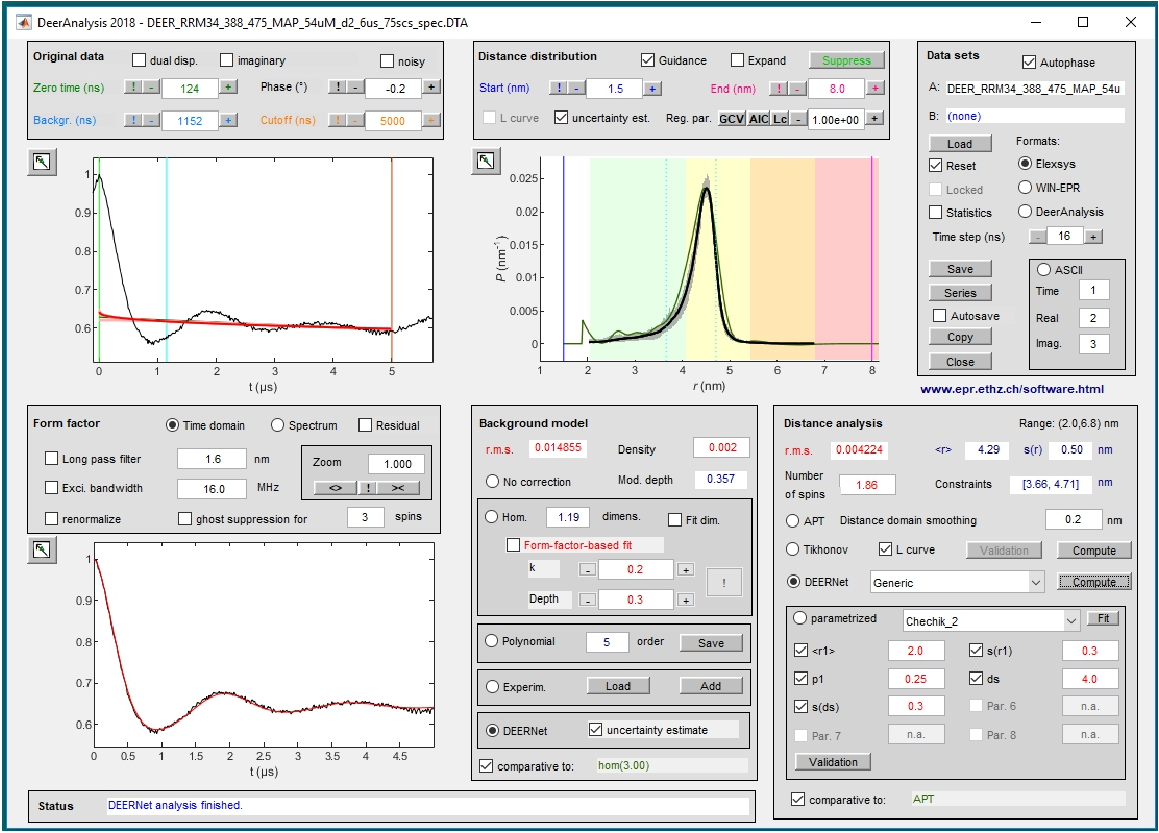
\includegraphics[width=0.95\textwidth]{fig1.pdf}
	\end{center}
	\caption{Graphical user interface of DeerAnalysis 2013.}
	\label{fig:manfig1}
\end{figure}

The user interface has been programmed with the following ideas in mind

\begin{tabular}{ll}
\noalign{\smallskip}
$\bullet$ & no {\em unnecessary} complexity \\
$\bullet$ & no hidden functionality (no menus) \\
$\bullet$ & default behavior should give reasonable results for most data \\
$\bullet$ & experienced users can easily override default behavior. \\
\end{tabular}


Default behavior is to read Elexsys (Xepr) data files, assume that the last three quarters of the data can be used for the background fit, adjust the phase automatically, and correct for exponential background decay (homogeneous spatial distribution of nanoobjects). Initially, no points are cut off at the end of the data set, the distance distribution is obtained by approximate Pake transformation (APT) \cite{jeschke2001}, and the mean distance $\left\langle r \right\rangle$ and standard deviation $\sigma_{r}$ by moment analysis within the range from 1.5 to 8 nm using distance domain smmothing with a filter width of 0.2 nm. A suggestion for cutting off noisy or distorted data points at the end of the data set is made. All this happens automatically once you load a data set via the {\ttfamily Load} button.

Different models for the background can be selected in the {\ttfamily Background models} panel (center of bottom half of Fig. \ref{fig:manfig1}) as described in more detail below. Similarly, Tikhonov regularization or fitting of the data by a model distance distribution can be selected in the {\ttfamily Distance analysis} panel. As these approaches are time-consuming, fitting is not started automatically but only after clicking on the corresponding {\ttfamily Fit} button. Adjustable parameters can be edited directly (the most common errors, such as non-digit input or values out of range, are corrected automatically) or incremented or decremented by {\ttfamily +} and {\ttfamily -} buttons, respectively. Several parameters can be adjusted or reset by automatic procedures (described below). This is done with the {\ttfamily !} buttons.

Display in each of the plot windows can be toggled. In the plot below the {\ttfamily Original data} panel display of the imaginary part (magenta trace) can be switched on or off by clicking on the {\ttfamily imaginary} checkbox. If two data sets have been loaded, the real part of the previous set (data set B) can be displayed as a blue trace by clicking on the {\ttfamily dual display} checkbox. This automatically suppresses display of the imaginary part of the active data set (data set A) and changes the {\ttfamily imaginary} checkbox into a {\ttfamily mod. depth scaling} checkbox. Dual display and modulation depth scaling also effect the other two plots, where results corresponding to data set B are also displayed as blue traces.

The plot below the {\ttfamily Dipolar evolution} panel can be toggled between time-domain display and display of the dipolar spectrum by checking the corresponding radiobuttons. Finally, the plot below the {\ttfamily Distance distribution} panel can alternate between display of the distance distribution and the L curve, after a Tikhonov regularization with L curve computation has been performed.

There is no Help function, but the controls are provided with short explanations that will show up when you move the cursor above them. 

\section{Pre-processing}
\label{preprocess}

\begin{figure}[ht]
 	\begin{center}
  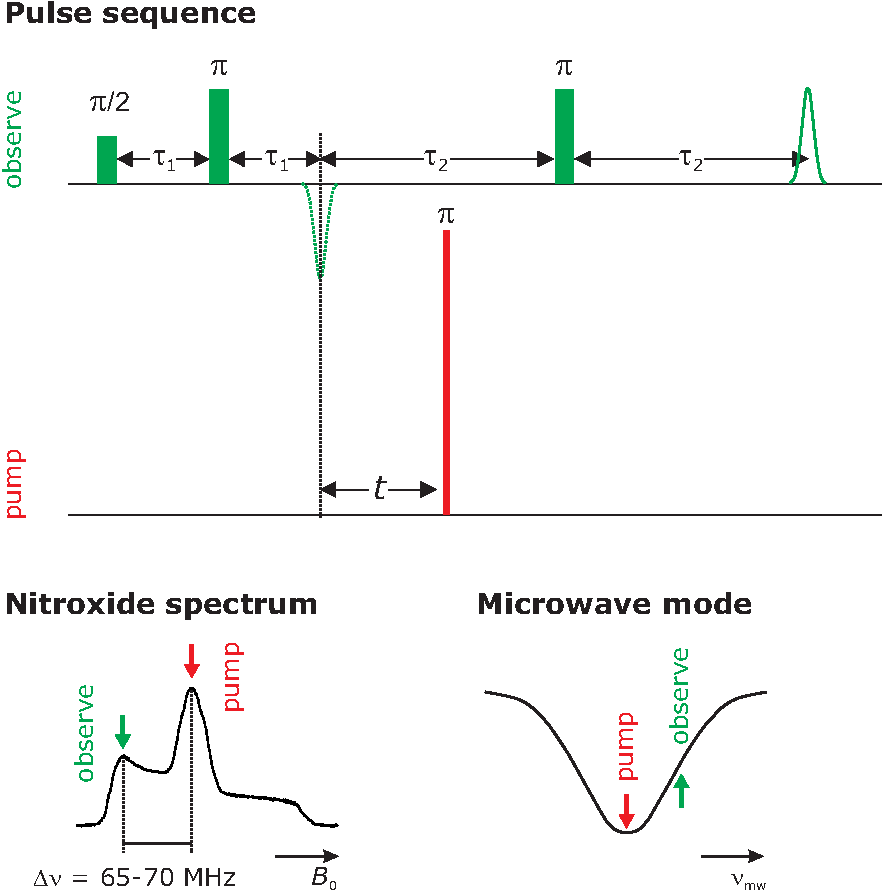
\includegraphics[width=0.8\textwidth]{fig2.pdf}
	\end{center}
	\caption{Pulse sequence and positions of the observer and pump frequency with
respect to the nitroxide spectrum and to the microwave mode for the four-pulse
DEER experiment.}
	\label{fig:manfig2}
\end{figure}

\subsection{Loading data}
Data input and output is initiated by buttons in the {\ttfamily Data sets} panel. By default the program expects Bruker Elexsys data (binary format). It recognizes
automatically if the data are complex (quadrature detection) or real
(single-channel detection, discouraged). If the data set is one-dimensional, it
is interpreted as output of a (classical) constant-time DEER experiment \cite{pannier2000}, see also Fig. \ref{fig:manfig2}.
If the data set is two-dimensional with exactly two traces, it is interpreted as
a variable-time DEER experiment \cite{jeschke2004b} with the first trace being the reference
trace and the second trace being the recoupled trace. For any other size of
experimental data, program response is undefined. If you unintentionally load
a data set of some other experiment, it is advisable to close the program and
restart it.

Mainly as a support for ESP 380 machines, the program has the capability
to read data in WIN-EPR binary format (select by radio button in the {\ttfamily Formats}
column of the). As the binary number format of the ESP 380 is somewhat obscure,
this mode requires that the data are first read into WIN-EPR on a PC and
saved again from WIN-EPR. This mode is less well tested than the Elexsys
mode and completely untested for two-dimensional data. Alternatively you can
convert ESP 380 data to ASCII data (also possible in WIN-EPR with command
sequence {\ttfamily 1D processing/Parameters/List data file.../Save}).

From an ASCII file, only one-dimensional data can be read. If there are
any header lines before the numerical data, they must start with a percentage
character (\%). By default, the program expects the time axis (in nanoseconds)
in the first column, the real part of the data in the second column, and the
imaginary part (if present) in the third column. These assignments can be
adapted in the edit fields below the {\ttfamily ASCII} radio button. For ASCII data
exported from WIN-EPR, the proper settings are 2, 3, and 4 instead of 1, 2,
and 3. The first six lines (header lines) have to be deleted or commented out by
a \% character. The program automatically recognizes if there is no imaginary
part. After successfully loading data, the {\ttfamily Status} panel shows a short characterization of the data set (const-time/variable-time
DEER, complex/real, number of data points). The filename is included in the
title of the DeerAnalysis main window and is also shown in line {\ttfamily A:} of the {\ttfamily Data sets} panel.

From version 2013 on, data saved by DeerAnalysis can be reloaded, when the {\ttfamily DeerAnalysis} radiobutton in the {\ttfamily Data sets} panel is activated. By default this activates the {\ttfamily Locked} checkbox in the same panel. Any of the DeerAnalysis output files (e.g. {\ttfamily ...\_bckg.dat}) can be selected, data from all files are loaded. The same feature allows for loading output data from the DEER window of MMM, provided that a comparison of experimental data with a simulated distance distribution was performed in MMM. In {\ttfamily Locked} mode any automatic processing is switched off, data and results are displayed in the form found in the saved files. The {\ttfamily Locked} checkbox can be deactivated to allow for data processing. Note however that not the full information from the primary data set is available after such reloading. Only the real part of the primary data, starting at the zero time determined by DeerAnalysis or by the user is saved and can be reloaded. In other words, phase correction and zero time determination should not be changed in such data sets.

\subsection{Determining zero time}
The time origin of the dipolar evolution function corresponds to $\tau_1 = \tau_2$ (see
Fig. \ref{fig:manfig2}). Because pulse lengths are finite, the relation between this equation and actual delays in the pulse sequence may not be trivial. We therefore suggest
determination of the time origin (zero time) from experimental data with a good
signal-to-noise ratio (SNR) for the pulse lengths and $\tau_1$ delay that you actually
use. To obtain a precise value a standard sample with a short distance should be used. If you later measure on the same spectrometer with the \emph{same} pulse lengths
and $\tau_1$ you can use the same value. Knowing this value is important for data
with poor SNR where automatic determination is likely to fail.
Automatic determination of zero time $t_0$ is based on the expectation that
the real part of the signal should be symmetric about the time origin. For the
proper choice of $t_0$, the first moment of the signal in a range symmetric about
$t_0$ should thus be zero. In a first step, the program approximates zero time by
the time $t_{\mathrm{max}}$ at which the real part is maximum. Then the first moment is
determined in a window $t_x<t_{\mathrm{max}}/2$, where $t_x$ is shifted through the whole data
set. The optimum value of $t_0$ is the time $t_x$ where the first moment is minimum. This procedure is performed with a time resolution of 1 ns, obtained by interpolation of the experimental data. Such enhanced time resolution improves results for very short distances, where it may be important that the true zero time may fall in between two experimental data points. Zero time is influenced by pulse lengths \cite{maryasov2000,milov2004}. This
algorithm should work well for good SNR an distances up to $\approx5$ nm. If it fails
under such conditions, $\tau_1$ is too short (expected symmetry of the data is spoiled
by interference between adjacent microwave pulses). The algorithm may fail
for very long distances where data close to the maximum are pretty flat. For
such long distances small mis-settings have only minor influence on the distance
distribution.

You may correct the automatically determined zero time by the {\ttfamily +} and {\ttfamily -}
buttons right and left from the value or by direct input of a new value in the edit field
(fit by the eyes). A wrong choice may be easier to detect when you switch
the {\ttfamily Dipolar evolution} plot to frequency domain ({\ttfamily spectrum}).

\subsection{Phase correction}
In a properly adjusted DEER experiment, the signal should be entirely in the
real part of the data set. If receiver offsets are canceled by [(+x)-(-x)] phase
cycling of the first pulse, as we strongly suggest, the imaginary part is zero. It is
therefore tempting to acquire and process only the real part. We discourage this.
For very weak signals, as you occasionally encounter with membrane proteins,
it is difficult to adjust signal phase exactly during setup. Consequently, part of
the signal will be in the imaginary part. Furthermore, depending on stability
of your spectrometer, there may be small phase drifts during the experiment.
It is better to correct for these drifts than to ignore them. Finally, unexpected
artifact signals are likely to manifest in the imaginary part (see Fig. \ref{fig:manfig3}). If the imaginary part \emph{after} phase correction strongly deviates from zero at early times,
it is advisable to acquire data with a longer $\tau_1$ value (see Fig. \ref{fig:manfig2}).

\begin{figure}[ht]
 	\begin{center}
  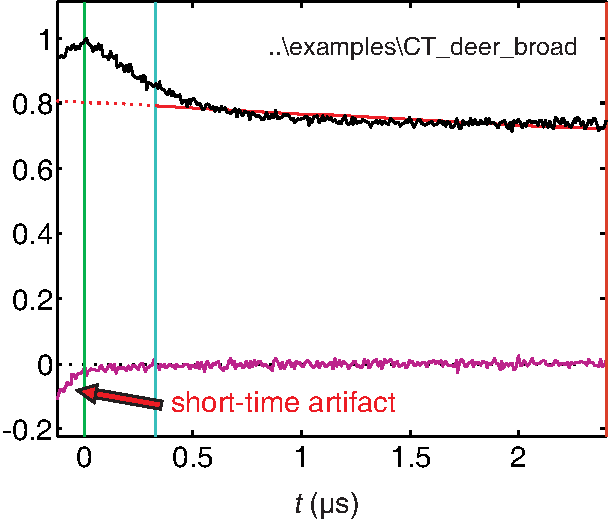
\includegraphics[width=0.5\textwidth]{fig3.pdf}
	\end{center}
	\caption{Imaginary-part artifact at early times (see red arrow) due to mw pulse
interference. Interpulse delay $\tau_1$ should
be long enough for the artifact to have almost completely decayed at $t = 0$
(green vertical line).}
	\label{fig:manfig3}
\end{figure}

Automatic phase correction can be based on the expectation that the imaginary
part should be zero at sufficiently long times. By default, the program
determines the corresponding phase correction directly after loading complex
data by minimizing the root mean square deviation of the imaginary part for
the last three quarters of the data (part between the blue and orange cursors). The phase
correction in degree is displayed in the {\ttfamily Original
data} panel.

You may correct phase manually by using the {\ttfamily +} and {\ttfamily -} buttons right and left from the value or by direct input of a new value in the edit field. Phase is automatically restricted to the range $(-180,+180)^\circ$. If you did not phase cycle
and do have a receiver offset, you may aim to flatten the imaginary part and
put all modulation into the real part. Note however, that in this case you are
likely to have a receiver offset in the real part, too. This will be detrimental to
data analysis. Automatic phase correction can be reactivated by the {\ttfamily !} button left from the value. It will always relate to the part of the data between the blue and orange cursors. If you move any of these cursors, the result may differ from the result that you got directly after loading.

Automatic phase correction after loading can be deactivated by unselecting
the check box {\ttfamily Autophase} in the {\ttfamily Data sets} panel.

In some measurements of weak samples with some spectrometers we found that automatic phase correction did not work and that after a manual phase correction that brought all modulation into the real part, a flat non-zero imaginary part remained. Apparently the problem comes from overload of the videoamplifier during the pulse. Small residual constant offsets of the imaginary part may also result if the phase drifted significantly during the measurement. Such data are less reliable than data with zero offset in the imaginary part, in particular with respect to background correction, as there may also be an offset in the real part. However, if the hardware problem cannot be fixed, it may still be warranted to process the data and interpret them (with caution), in particular, as for weak samples the background may be flat, so that an offset in the real part does not pose a problem.

DeerAnalysis2018 automatically fits an offset in the imaginary part if the checkbox \texttt{Offset corr.} (below the \texttt{Load} button) is activated. The fitting happens on file load (if the checkbox \texttt{Reset} is also activated) and on clicking the \texttt{Phase($^{\circ}$) !} button in the \texttt{Original data} panel. The fit criterion is \emph{flatness} of the imaginary part in the last 87.5\% of the data points. The first 12.5\% are excluded to allow for early-time artifacts as shown in Fig. \ref{fig:manfig3}. Alternatively, you can use manual phase correction to flatten the imaginary part "by eyes". The offset of the imaginary part is displayed as a magenta dotted line. If you obtain large offsets or visible offsets even for strong samples, please fix your spectrometer.

\subsection{Cutting data}
For several reasons, you may want to exclude points at the end of
your data set from analysis. First, some people prefer to acquire data up to
delays $t$, where the pump pulse starts to interfer with the last observer pulse
or even overlaps with it. In this case, the last data points are spoiled. Second,
if at maximum $t$ the signal has decayed to a very small value (say 0.1 times
maximum intensity), the dipolar eveolution function after background correction
will be rather noisy, as correction involves division by the background decay.
Third, SNR in variable-time DEER data increases with $t$ even before background
correction. It may be wise to cut the data at a time where noise is still tolerable.

By default no data points are cut off at the end, but a suggestion for cutoff is displayed as an orange vertical cursor in the {\ttfamily Dipolar evolution} plot (see Fig. \ref{fig:manfig4}). This suggestion is derived from the difference $D$ between the experimental dipolar evolution function and its fit by the APT result. The mean square deviation $M_k$ of eleven consecutive points $D_{k-5}\ldots D_{k+5}$ around the $k$th data point is computed for all indices $k$. The minimum of $M$ is a measure for the noise level. An acceptable noise level of $6\mathrm{min}(M)$ is assumed. The programm then searches for a range of consecutive points at the end of the data set that \emph{all} fulfil the condition $M(k)>6\mathrm{min}(m)$. If such a range of points exists, the program suggests to cut it off. Otherwise the orange cutoff cursor is set to the end (right border) of the trace.

\begin{figure}[ht]
 	\begin{center}
  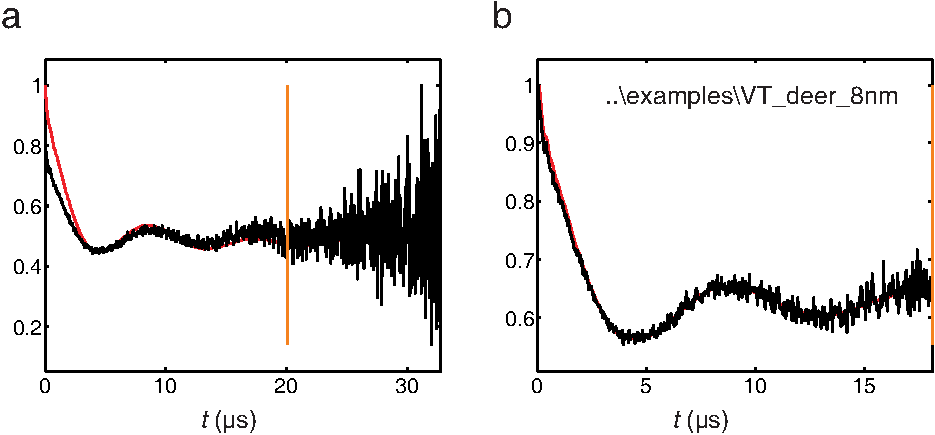
\includegraphics[width=1.0\textwidth]{fig4.pdf}
	\end{center}
	\caption{Cutting off the noisy part at the end of variable-time DEER data. (a) {\ttfamily Dipolar evolution} plot for the whole data set. The orange cursor shows the suggested cutoff time. (b) Dipolar evolution function (black) and
fit (red) by a distance distribution obtained with APT after cutting the data at the suggested time.}
	\label{fig:manfig4}
\end{figure}

The suggestion can be accepted by clicking on the {\ttfamily !} button of the {\ttfamily Cutoff} controls in the {\ttfamily Original data} panel. Note that this may in turn improve the fit, thus leading to a smaller value $\mathrm{min}(M)$ and a new cutoff suggestion. Therefore, it is advisable to click on the {\ttfamily !} button several time to iteratively approach the optimum cutoff. Furthermore, the cutoff suggestion depends on correct settings of other parameters (zero time, phase). For instance, for the variable-time DEER data set shown in Fig. \ref{fig:manfig4} the zero time must be zero, while the program automatically determines 96 ns. If this is not corrected, not good fit is obtained and unnecesserily many data points are cut off. Note also that this data set with relatively poor SNR was intentionally selected for explanation of data cutoff. For many data sets, no cutoff at all may be required and DeerAnalysis2018 immediately sets the cutoff cursor to the right border.

Generally, cutting off a significant amount of data will suppress noise but will also cause a suppression of long distances by background correction. Proper background correction may
become more difficult. 
 
\subsection{Background correction}
In most cases, EPR distance measurements are performed to elucidate the structure
of a nanoscopic object. Only distances within this object are of interest.
The contribution of distances to neighboring objects should be suppressed. If
you think about a biradical or bilabelled protein molecule, you want to measure
the intramolecular distance and suppress contributions from intermolecular
distances.

Such a separation of the signal $V(t)= \{ 1 - [1 - \Delta D(t)] \} B(t)$ into a dipolar evolution function $D(t)$ for the
nanoobject itself and a background decay $B(t)$ due to neighboring objects requires a
criterion for distinguishing the two contributions. Furthermore, the functional
form of the background decay has to be known. This functional form is related to
the spatial distribution of the nanoobjects. A separation can only be successful
if distances within the object are typically shorter than distances to neighboring
objects. The wanted contribution is then confined to the earlier part of the time domain
data, while later parts are dominated by the background decay. The
decay can only be fitted properly if the maximum time $t$ in the pulse sequence
(Fig. \ref{fig:manfig2}) is significantly longer than the time at which the dipolar modulation
has decayed. A more detailed discussion can be found in Ref. \cite{jeschke2004a}.

Separation into the two contributions is simple and reliable if the distance
distribution is dominated by distances shorter than 4 nm. In protein samples, it
becomes challenging for distances between 4 and 6 nm, and near to impossible
for distances longer than 6 nm, unless protons around the spin labels can be
strongly diluted by deuteration \cite{jeschke2004b}. Note that one can still get a quite reliable estimate of a distance of closest approach if separation fails. However, the
width and shape of the distance distribution should not be discussed in such 
a situation. 

In simple cases (short distances and homogeneous distribution of the nanoobjects
in three dimensions), separation depends only weakly on the choice of parameters.
Default behavior of the program should then be sufficiently good.
By default, an exponential background decay corresponding to a homogeneous
three-dimensional distribution is fit to the last three quarters of the data. The
fit parameter is the decay time constant, which is proportional to the concentration
of nanoobjects. With proper calibration such fits can be used to determine
local concentrations (see Section \ref{localconc}).

Generally, the background is shown as a red line in the {\ttfamily Original data} plot. A continuous line is plotted in the range where the background was fitted (between the blue and orange cursors), a dotted line is plotted where the fit was extrapolated. The r.m.s. value of the background fit is displayed in the {\ttfamily Background model} panel.

\begin{figure}[ht]
 	\begin{center}
  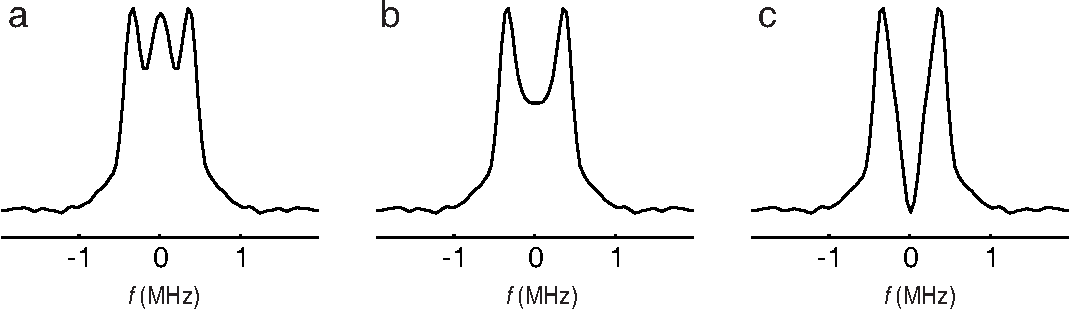
\includegraphics[width=1.0\textwidth]{fig5.pdf}
	\end{center}
	\caption{Manifestation of different background fits in the dipolar spectrum
(example data set CT\_DEER\_5nm). (a) Part of the background is attributed to
the biradical. (b) Good separation of intra- and intermolecular contributions,
as obtained with automatic correction ({\ttfamily !} button). (c) Part of the biradical
contribution is attributed to the background.}
	\label{fig:manfig5}
\end{figure}

For distances of $\approx4$ nm and longer, choice of the time range for background
fitting may decide whether you obtain artifacts in the distance distribution at
long distances. Unlike the other problems in determining a distance distribution,
this problem is most severe for narrow distributions of distances. In this case the
modulation decays more slowly and thus interferes more strongly with the background
fit. Our automatic determination of the optimum fit range is based on
the assumption that the longest detectable distance exceeds the largest distance
within the nanoobject. If this condition is met, the distance distribution after
correct background correction is zero at the maximum detectable distance. This
can be checked by approximate Pake transformation (APT, see below). APT is
sufficiently fast to be applied at all possible choices of the starting time for the
background fit. For any selected background model, this search for the optimum
starting time can be initiated by clicking on the blue {\ttfamily !} button in
the {\ttfamily Original data} panel. Depending on the length of your data set and the
speed of your computer, this optimization can take up to a few minutes.

The starting time for background fitting can also be adjusted manually with
the blue {\ttfamily +} and {\ttfamily -} buttons or by direct input into the edit field. The consequences can best be judged when switching the bottom left plot below to frequency
domain. For a narrow distance distribution, the black trace should look like
a Pake pattern. Deviations are best seen at zero frequency. There should be
neither a positive spike nor an obvious hole in the center of the Pake pattern
(see Fig. \ref{fig:manfig5}).

Background correction can be switched off completely by selecting the {\ttfamily No
correction} radiobutton in the {\ttfamily Background model} panel. In this modus the input data are interpreted as a dipolar evolution function which is already separated from background. The
modus is intended for compatibility with external pre-processing programs,
for polynomial fitting of single-label data to derive an experimental background
function (see below), or for fitting by a user model that explicitly contains the background contribution. User models consisting of a single Gaussian peak with 3D homogeneous background ({\ttfamily Gaussian\_hom}) or of two Gaussian peaks with 3D homogeneous background ({\ttfamily 
Two\_Gaussians\_hom}) are already included in DeerAnalysis2018. However, we strongly discourage fitting background and distance distribution simultaneously, as such fits are very likely to end up in local minima of the error hypersurface. Whenever a separation of the background contribution from the contribution of the nanoobject can be performed with some confidence, it should be done before analysis of the distance distribution.

For long distances, the intramolecular contribution may be significant throughout the whole time range. In such cases, any fit of a background function to the data is biased. If independent information on expected modulation depth and concentration (density) is available, e.g. from other double mutants of the same protein, it may be better to directly input these estimates instead of fitting. This can be done by selecting the option {\ttfamily Form factor based fit}. This option is displayed red when the program estimates from the preliminary distance distribution that fitting would be more reliable and is displayed green if the program expects problems with background fitting. 

It is also possible to systematically vary modulation depth and density and search for the values that lead to the best fit of the form factor. The rational behind this algorithm is that the background contribution cannot be fitted by a distribution of distances with an upper limit. Incomplete background correction or overcorrection will thus lead to a deterioration of the fit of the form factor. This algorithm works well for data with very high signal-to-noise ratio, but is easily mislead by noise. It should thus be used with caution. The search for optimum modulation depth and density can be started by selecting the option {\ttfamily Form factor based fit} and then clicking on the {\ttfamily !} button in the {\ttfamily Form factor based fit} subpanel.

If there are uncertainties about the parameters of background correction, the result of Tikhonov regularization should be checked by using the {\ttfamily Validation} module. 

In the following we shortly discuss the possible choices for the spatial distribution
of nanoobjects. They can be selected by checking the corresponding radiobutton in the {\ttfamily Background model} panel.

\subsubsection{Homogeneous}
This model is strongly suggested for all cases where you do not have experimental background functions from singly labelled molecules. The general background function in this model is
\begin{equation}
	B \left( t \right) = \exp \left( -(k t)^{d/3} \right) 
\end{equation}
where $k$ depends on the density of the spins and the pump pulse inversion efficiency, and $d$ is the dimensionality of the homogeneous distribution. Unless there is a confinement on length scales below 10 nm, the distribution is homogeneous in $d=3$ dimensions. This case applies to most solutions. Membrane proteins in a liposome may be confined to $d=2$ dimensions. If possible, such confinement should be established by control measurements on singly labelled proteins, for which $d=2$ is expected give a better fit than $d=3$. For labels attached to a stretched polymer chain, $d=1$ may be appropriate. Note also that a choice of $d=6$ corresponds to a Gaussian background decay, as it has been observed with the single-frequency SIFTER experiment \cite{sifter}. The dimension is not necessarily an integer number- if experimental data of a singly labelled sample can be nicely fitted with a fractal dimension, it is advisable to use the same fractal dimension for background correction of the corresponding doubly labelled sample.

When the {\ttfamily Fit dimensionality} checkbox is selected, both $k$ and $d$ are fitted. This mode is suggested only for determining the fractal dimension of purely homogeneous (singly-labelled) samples. In this case the {\ttfamily Bckg.} control in the {\ttfamily Original data} panel should be set to zero (green and blue cursors coincide), as the early decay of the data is most sensitive to the parameter $d$.   

\subsubsection{Polynomial}
Short distances are underrepresented in the intermolecular distance distribution, ff the spin labels are attached to nanoobjects that cannot penetrate each other. As a result, the intermolecular contribution decays more slowly at early times than would be expected for a homogeneous distribution. If singly labelled objects are available, the intermolecular part can be measured separately and an experimental background function can be derived. Directly using the noisy experimental data set of the singly labelled sample would introduce significant statistical errors. It is therefore prudent to use a smooth fit function for that purpose.

Almost any intermolecular decay can be reproduced by fitting a polynomial to the \emph{logarithm} of the original data. DeerAnalysis2018 allows for polynomials with an order of up to 15, but note that the lowest order should be selected that still gives a good fit (flat trace in the {\ttfamily Dipolar evolution} plot. Polynomial fits are mainly implemented for deriving and afterwards saving experimental background functions from singly labelled samples, not for direct background correction.

\subsubsection{Experimental}
Once experimental background functions have been derived from singly labelled samples, they can be used for correcting the background in corresponding doubly labelled samples. In this mode, the relative magnitudes of the polynomial coefficients are kept fixed. The background model is given by
\begin{equation}
	B \left( t \right) = \exp \left( -k \sum _{n=0} ^o c_n t^n \right)
\end{equation}
where $k$ is the density (concentration) parameter, $o$ the order of the polynomial, and the $c_n$ are the polynomial coefficients determined previously on the singly labelled samples. The only fit parameter is $k$.

In principle, background data should be individually measured for both label positions in a doubly labelled sample, as the supression of short distances depends on how deep the label is buried in the nanoobject. The weighted sum of both background functions is a better approximation for the actual background in the doubly labelled sample than each individual background function. Several background polynomials can be added using the {\ttfamily Add} button in the {\ttfamily Background model} panel. A weighting factor can be specified in a dialog box that opens after clicking on this button. Note that the different labeling efficiencies at the two positions are already accounted for with weighting factor 1.0 if both singly labelled samples were measured with the same protein concentration. 

\subsection{Determining local concentrations}
\label{localconc}
The parameters of the background fit are related to the number of coupled spins
within the nanoobject (modulation depth after background correction) and to the density of nanoobjects (parameter $k$). For calculation of the number of spins and of absolute densities, the modulation depth parameter $\lambda$ has to be known, which depends strongly on the
excitation position, length, and flip angle of the pump pulse and weakly on line broadening in the nitroxide spectrum and shape of the resonator mode. Reliable
quantification therefore requires a calibration with known samples and proper
adjustment of the flip angle of the pump pulse (see Section \ref{experimental}). The calibration should
be repeated if the resonator or the length of the pump pulse is changed. Protonated
and deuterated nitroxide spin labels also require separate calibrations.
Determination of the number of coupled spins is more reliable when based on
Tikhonov regularization or a fit of the data by a model distribution and is therefore discussed later on (Section \ref{numspins}).

For a 3D homogeneous distribution of objects, the density is proportional to
the local concentration. The term local refers to the length scale of the DEER
experiment, which extends to approximately 10-20 nm for the background.
Measurements of local concentrations can be calibrated with a solution of an
appropriate spin label (e.g., protonated or deuterated TEMPOL) in toluene.
An example data set from our own calibration (CT\_DEER\_tempol\_2500uM) is
provided. This data set was acquired with a 2mM TEMPOL solution in toluene,
which corresponds to a concentration of 2.5 mM at 80 K, as toluene shrinks to
approximately 80\% of its room temperature volume when freeze-quenched in
liquid nitrogen.

To calibrate 3D background fitting for determination of concentrations, select
{\ttfamily Homogeneous} as the background model, set {\ttfamily dimensions} to 3, and load a data set for a sample with known concentration. Adjust zero time and phase, if necessary. Now input
the concentration (in the units you prefer) into the edit field {\ttfamily Density}. The color of the density value then changes to green. When you now load other experimental data sets that have
been measured with the same resonator and experimental settings and use the same background model, you can directly read off concentrations
from the edit field {\ttfamily Density}. Note that the program looses calibration on
restart.

\subsection{Long-pass filtering}
The major artifact contribution to DEER time-domain signals is usually nuclear
modulation due to matrix protons. At X-band frequencies, such proton modulation
corresponds to a distance of approximately 1.5 nm. By restricting the distance range for analysis to (1.75, 8) nm, contributions by nuclear modulation can be suppressed. However, as computation of distance distribution is an ill-posed problem, an out-of-range artifact may
still influence the result within the range of interest. Very strong proton modulations,
as they are sometimes encountered for membrane proteins in liposomes
or detergent micelles, should thus be eliminated by filtering.

This can be achieved by completely eliminating contributions above a certain
maximum frequency, which roughly corresponds to suppressing distances
below a certain minimum distance. Such complete suppression was described in
Ref. \cite{jeschke2004b}. For broad distance distributions with contributions both below and above 1.75 nm, complete suppression may introduce an artificial hole at $t = 0$ into the time-domain data and may thus replace the nuclear modulation artifact with a suppression
artifact. To avoid this, filtering in DeerAnalysis2018 is performed by fitting a third-order polynomials to the real and imaginary parts of the frequency-domain data between
the cut-off frequency and the Nyquist frequency. The frequency-domain data
in this range are then replaced by the polynomial. This suppresses the sharp
nuclear modulation peak as well as high-frequency noise, while keeping the high frequency
contributions of broad distance distributions intact.

Filtering is enabled by selecting the {\ttfamily Long pass filter} checkbox in the
{\ttfamily Dipolar evolution} panel. The cut-off distance (lower limit, default
1.6 nm) can be changed in the edit field right from this check box. When
working with broad distributions of short distances, the default value is often a
good compromise between residual proton modulation and partial suppression
of short distances.

\section{Extracting distance distributions}
\label{distribution}

\subsection{General remarks}
The computation of a distance distribution $P(r)$ from a dipolar evolution function
$V(t)$ is an ill-posed problem. For such problems, small variations in the
input data (e.g., noise) can cause large variations in the output data. In other
words, significantly different distance distributions may correspond to very similar
dipolar evolution functions. Data analysis therefore depends strongly
on striking a good compromise between improving resolution and decreasing the
influence of experimental noise. First
and foremost, data should be acquired with as good as possible SNR. Reproducing
results for a given sample is usually a good idea. Second,
ill-posedness must be taken into account in data analysis. There are several
ways of doing this, which all have one feature in common: one tries to find a
resolution in distance domain at which a good fit of the experimental data is
obtained without introducing strong noise artifacts into the distance distribution.

\subsection{Reliability of distance distributions}
\label{reliability}
The reliability of distance distributions depends strongly on the maximum dipolar evolution time. 
A rule of thumb was derived by reanalyzing data that were simulated from known distance distributions.
At a maximum dipolar evolution time $t_\mathrm{max} = 2 \ \mu$s the shape of the distance distribution is
reliable up to a distance of about 3 nm (reliable distribution limit). The mean distance $\langle r \rangle$ and width $\sigma_r$ are 
reliable up to a distance of 4 nm (reliable width limit), whereas the mean distance, but not the width is reliable between 4 and 5 nm
(reliable meand distance limit). Beyond 5 nm no reliable mean value can be determined, although the presence of a long distance 
(distinct from background) can be recognized up to 6 nm (distance regonition limit). All these limits scale with the cubic root of $t_\mathrm{max}$.

\begin{figure}[ht]
 	\begin{center}
  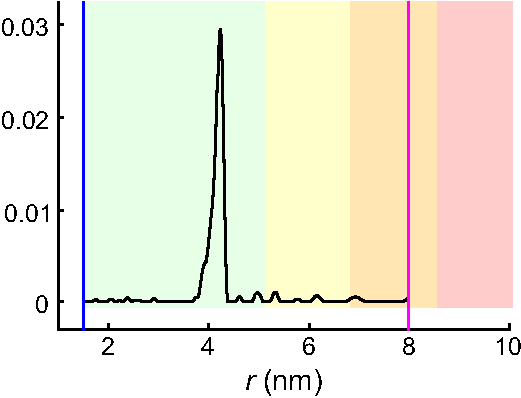
\includegraphics[width=0.5\textwidth]{fig_reliability.pdf}
	\end{center}
	\caption{Color coding for reliability ranges. Pale green: Shape of distance distribution is reliable. Pale yellow: Mean distance and width are reliable. Pale orange: Mean distance is reliable. Pale red: Long-range distance contributions may be detectable, but cannot be quantified. The example data were cut off at a maximum dipolar evolution time of 10 $\mu$s. In this particular case the shape of the distribution can safely be interpreted.}
	\label{fig:reliability}
\end{figure}

DeerAnalysis2018 displays reliability ranges by color-coding the background of the distance distribution plot. The pale green range
corresponds to a reliable shape of the distribution, the pale yellow range to reliable mean distance and width, the pale orange range to 
reliable mean distance (but not width), and the red range to recognition of a long-distance contribution that cannot be quantified. The computed distribution is displayed only up to the distance recognition limit.

This new feature is intended to caution users against overinterpretation of data. For preparing figures of distance distributions for papers it may be required to suppress these background colors. This can be achieved by deactivating the checkbox {\ttfamily Guidance}.

\subsection{Approximate Pake Transformation (APT)}
A very fast algorithm relies on an approximate integral transformation to
dipolar frequency domain, subsequent correction of cross-talk artifacts, and
mapping to distance domain (APT) \cite{jeschke2001}. Ill-posedness is moderated by proper
discretization in dipolar frequency domain. If SNR is too small, the distance
distribution may still be influence by strong noise artifacts. A better
compromise between reliability of the distribution and resolution can then be
achieved by distance-domain smoothing, i.e., by giving up resolution in favor
for a smoother distribution. As APT is very fast, it can also be used to generate
starting values for fit procedures. The disadvantage of APT with respect
to other techniques is that it cannot incorporate the constraint $P(r) > 0$ (for
all $r$). This disadvantage, however, is significant, as the constraint strongly
stabilizes the solution. For this reason, several other approaches for data analysis
are incorporated into DeerAnalysis2018.

\subsection{Tikhonov regularization}

Other approaches rely on computation of a simulated time-domain signal $S(t)$ from
a given distance distribution $P(r)$ by
\begin{equation}
	S \left( t \right) = K \left( t, r \right) P \left( r \right) ,
\end{equation}
where $K$ is the kernel function. For the DEER experiment with ideal pulses, the kernel function is known analytically
\begin{equation}
	K \left( t, r \right) = \int _0 ^1 \cos \left[ \left( 3x^2-1 \right) \omega_{\mathrm{dd}} t \right] \mathrm{d}x \; ,
	\label{eq:ideal_kernel}
\end{equation}
with
\begin{equation}
	\omega_{\mathrm{dd}} \left( r \right) = \frac{2 \pi \cdot 52.04 \; \mathrm{MHz} \; \mathrm{nm}^{-3}}{r^3} \; .
\end{equation}
The case of non-ideal pulses is discussed in Section \ref{bandwidth}.

The most elegant response to ill-posedness is Tikhonov regularization. In this approach, the compromise between smoothness (artifact suppression) and resolution of the distance distribution is quantified by a regularization parameter $\alpha$. The optimum distance distribution $P(r)$ is found by minimizing the objective function
\begin{equation}
	G_{\alpha} \left( P \right) = \left\| S \left( t \right) - D \left( t \right)  \right\|^2 + \alpha \left\| \frac{\mathrm{d}^2}{\mathrm{d}r^2} P \left( r \right) \right\|^2
	\label{eq:regul}
\end{equation}
for a given $\alpha$. The first term on the right hand side of eqn (\ref{eq:regul}) is the mean square deviation between the simulated and experimental dipolar evolution function while the second term is the regularization-parameter weighted square norm of the second derivative of $P(r)$, which is a measure for the smoothness of $P(r)$. The larger $\alpha$ the less noise artifacts are introduced. However, a larger $\alpha$ also causes a stronger broadening of peaks in the distance distribution. Therefore, small $\alpha$ are required for samples with well defined distances (narrow peaks) and large $\alpha$ for very broad distributions, which otherwise disintegrate into many narrow peaks. Unfortunately, the correct width of the peaks is often not known in advance.  

There are different ways for mathematically defining an optimum regularization parameter. The past version DeerAnalysis2004 used the self-consistency criterion \cite{honerkamp1990, weese1992}. However, determination of an optimum $\alpha$ is itself influenced by noise \cite{jeschke2004a}, and the self-consistency criterion appears to be more sensitive to noise distortions than the L curve criterion \cite{freed2005}. The L curve is a plot of $\log \eta ( \alpha )$ versus $\log \rho ( \alpha )$, where 
\begin{equation}
	\rho \left( \alpha \right) = \left\| S \left( t \right) - D \left( t \right)  \right\|_{\alpha}^2
\end{equation}
quantifies the means square deviation and
\begin{equation}
	\eta \left( \alpha \right) = \left\| \frac{\mathrm{d}^2}{\mathrm{d}r^2} P \left( r \right) \right\|_{\alpha}^2
\end{equation}
the smoothness. For well behaved data (good signal-to-noise ratio, relatively narrow peaks in the distribution), this plot is L-shaped as is illustrated in Fig. \ref{fig:manfig6}a. In the range of small regularization parameters $\alpha$ (left of the corner, undersmoothing) the slope is steep and negative, as increasing $\alpha$ and thus the smoothing strongly decreases the norm of the second derivative of $P(r)$ without strongly affecting the mean square deviation. In contrast, right of the corner (oversmoothing) the mean square deviation increases strongly with increasing $\alpha$ as the simulation is no longer a good fit of the data. At the same time, $\eta$ decreases only gradually as noise-related spikes in $P(r)$ are already smoothed out. If the SNR is worse and the peaks in the distance distribution are broader, the corner of the L curve is somewhat less pronounced (Fig. \ref{fig:manfig6}b).

\begin{figure}[ht]
 	\begin{center}
  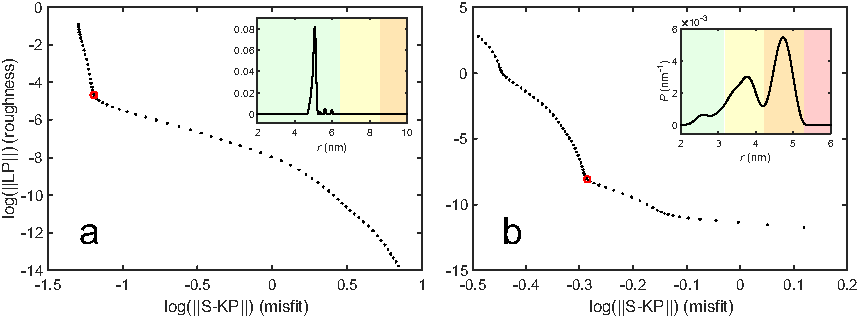
\includegraphics[width=1.0\textwidth]{fig6.pdf}
	\end{center}
	\caption{Tikhonov L curves. The red data points correspond to the optimum regularization parameter. The insets show the distance distribution obtained with this parameter. a) Data set dOTP\_5nm, $\alpha = 1$. b) Data set CT\_DEER\_broad, $\alpha = 100$.}
	\label{fig:manfig6}
\end{figure}

In DeerAnalysis2018 the L curve criterion is implemented for unconstrained Tikhonov regularization, which allows for very fast computation of the L curve. Initially, constrained Tikhonov regularization is computed only at the automatically detected corner of the L curve (red circles in Fig. \ref{fig:manfig6}). The user can click on other points in the curve and constrained Tikhonov regularization is then recomputed for the corresponding regularization parameter. For regularization parameters that do not correspond to the automatically detected corner, a blue circle is shown.

Tikhonov regularization is performed by clicking on the corresponding {\ttfamily Fit} button in the {\ttfamily Distance analysis} panel. By default, L curve computation is enabled, since the shape of the L curve contains information about the quality of the data, and because the extended $\alpha$ is needed for the automatic selection methods (L-curve corner, AIC, GCV - see below) to work. If it is too time consuming for a particular dataset, it can be switched off, which is however not recommended. The regularization parameter (default: 1) can be changed in the corresponding edit field in the {\ttfamily Distance distribution} panel. The distance range for Tikhonov regularization is determined by the blue and magenta start and end values in the {\ttfamily Distance distribution} panel, which can also be edited. Computation of the L curve can be requested by clicking on the {\ttfamily L curve} checkbox in the {\ttfamily Distance analysis} panel and subsequently clicking on the {\ttfamily Compute} button. The status line indicates the progress of the L-curve calculation. After the computation, the L curve is automatically displayed instead of the {\ttfamily Distance distribution} plot with the automatically derived selection of the L-curve corner highlighted in red and the corresponding regularization parmeter shown in the {\ttfamily Reg. par.} control. The selection of the regularization parameter can be shifted with the {\ttfamily +} and {\ttfamily -} buttons of the {\ttfamily Reg. par.} controls. Such changes update the fit in the {\ttfamily Dipolar evolution} panel and the r.m.s. value in the {\ttfamily Distance analysis} panel. The distance distributions for different regularization parameters can be inspected in the same way after unselecting the {\ttfamily L curve} checkbox in the {\ttfamily Distance distribution} panel.

Automatic L curve corner recognition selects the regularization parameter that has the shortest distance from the lower left corner in a log-log plot of square norm of the second derivative of $P(r)$ vs. mean square deviation of the simulated from the experimental form factor (new algorithm since DeerAnalysis2009). The lower left corner is defined by the minimum square norm of the second derivative of $P(r)$ and the minimum mean square deviation among all regularization parameters for which Tikhonov regularization was performed. Note that L curves can be misshaped if there are problems with background correction or if data are very noisy. In such cases the automatically determined choice of the regularization parameter may not be reasonable. If you have any information on the expected width of the distribution (or of the most narrow features in the distribution) from data other than the one being analyzed, it is usually best to select the regularization parameter manually. The optimum choice is the one that just does not cause undue broadening of expected narrow features.

Beside the L-cruve corner, DeerAnalysis2018 offers two additional methods for selecting an appropriate value of the regularization parameter $\alpha$, the Akaike information criterion (AIC) and the generalized cross-validaton (GCV)\cite{edwards2018}. Both can be obtained by clicking on the respective buttons labeled {\ttfamily AIC} and {\ttfamily GCV} next to the edit box for the regularization parameter. The L-curve corner value can be obtained again by pressing the button labeled {\ttfamily Lc}. The AIC method treats the solutions determined with different values for $\alpha$ as different models and determines the value that corresponds to the most parsimonious model. The GCV method drops one datapoint from the dataset at a time and determines $\alpha$ that generates a fit from the remaining datapoints that best recovers this dropped datapoint. This procedure is repeated for every datapoint in the DEER time trace. Whereas the L-curve corner method  tends to over-broaden the distance distributions, the AIC and GCV typically result in much sharper distributions, with a tendency to underbroaden. They also can fail of the tail of the DEER trace is not properly cropped.

After a Tikhonov regularization has been performed, the {\ttfamily Validation} button becomes accessible. An error analysis with respect to noise and uncertainties in background correction can now be performed (see Section \ref{validation}).

\subsection{User models}
Generally, the solution of an ill-posed problem can be stabilized by introducing additional constraints. A distance distribution $P(r)$ that conforms to a simple model with only a few parameters, for example a distribution consisting of one or two Gaussian peaks, is strongly constrained. Fitting of the data by a model distribution can thus improve reliability of the analysis. Furthermore, by comparing the parameters for a series of related samples trends can be easily recognized. This approach is offered in DeerAnalysis2018 by an interface for fitting pre-processed data by user-defined models for the distance distribution $P(r)$. Model functions with one and two Gaussian peaks are already implemented. The model library can be extended by the user as described below.

In applying this approach one should be aware that a model can impose constraints that do not apply to the true distance distribution and may thus suppress information contained in the original data. For instance, the example data set {\ttfamily dOTP\_5nm} can be fitted relatively well by a distance distribution consisting of a single Gaussian peak, but this imposes a symmetry on the peak that is not a feature of the true distribution. The true distribution decays more steeply towards high distances than towards low distances as seen in the inset in Fig. \ref{fig:manfig6}a (and the reason for this asymmetry is well understood). It is thus advisable to perform a model-independent analysis by Tikhonov regularization first. From a set of distance distributions for the same class of samples, it is then often possible to derive a model function that does not impose undue constraints but does make use of additional information on the sample that comes from other characterization techniques.

\subsubsection{Fitting with existing models}
\label{fit_existing}
When DeerAnalysis2018 starts, the program checks the subdirectory {\ttfamily models} for existing Matlab scripts (extension {\ttfamily .m}). The current distribution contains the scripts 
\begin{itemize}
	\item {\ttfamily Gaussian.m} \\ Single Gaussian peak with mean distance $\left\langle r \right\rangle$ and standard deviation $\sigma(r)$.
	\item {\ttfamily Gaussian\_hom.m} \\ Single Gaussian peak with mean distance $\left\langle r \right\rangle$ and standard deviation $\sigma(r)$. and homogeneous 3D background. To be used with {\bf Background model} {\ttfamily No correction} and only with great care.
	\item {\ttfamily random\_coil.m}. \\ Random-coil model for a polymer chain or an unfolded protein or an unfolded domain of a protein. $N$ is the number of amino acid residues between the two labels including both labeled
 residues. $\nu$ is the scaling exponent (0.602 for good solvents, expected for soluble proteins in water, 0.5 for $\theta$-solvent, less than 0.5 for poor solvents).
 	\item {\ttfamily Rice3d.m} \\ Single Rice peak \cite{koehler2011} with mean distance $\left\langle \nu\right\rangle$ and standard deviation $\sigma$ in three dimensions. Note that for the Gaussian limit of the Rice distribution, the standard deviation $\sigma$ is by a factor $\sqrt{2}$ smaller than the value of $\sigma$ in the Gaussian distribution as implemented in DeerAnalysis.
\item {\ttfamily Sphere\_Surface.m}. \\ Homogeneous distribution of spin labels on the surface of a sphere. The sphere diameter $d_s$ has a Gaussian distribution with standard deviation $\sigma(d_s)$. 
  \item {\ttfamily Triangle\_DGauss.m} \\ Assumes a three-spin system (equilateral triangle) with double Gaussian distribution of the center-vertex distance (two Gaussian peaks). Useful for homotrimers with two distinct conformations or significantly non-Gaussian distance distributions. Pair- and three-spin contributions to the form factor are considered, based on \cite{jeschke2009} with a correction in the fraction of two-spin contributions. The total modulation depth $\Delta$ (\texttt{Delta}) and the number of Monte Carlo trials (\texttt{nmc}) are fixed parameters, whereas $\Delta$  should be set to the modulation depth obtained with background fitting.  
  \item {\ttfamily Triangle\_Gauss.m} \\ Assumes a three-spin system (equilateral triangle) with Gaussian distribution of the distance between the center and the vertices. Useful for homotrimers. Pair- and three-spin contributions to the form factor are considered, based on \cite{jeschke2009} with a correction in the fraction of two-spin contributions. The total modulation depth $\Delta$ (\texttt{Delta}) and the number of Monte Carlo trials (\texttt{nmc}) are fixed parameters, whereas $\Delta$  should be set to the modulation depth obtained with background fitting.
	\item {\ttfamily Two\_Gaussians.m} \\ Two Gaussian peaks with mean distances $\left\langle r_1 \right\rangle$ and $\left\langle r_2 \right\rangle$ and standard deviations $\sigma(r_1)$ and $\sigma(r_2)$. The population of the first peak (integral) is $p_1$, the one of the second peak $1-p_1$.
	\item {\ttfamily Two\_Gaussians\_hom.m} \\ Two Gaussian peaks with mean distances $\left\langle r_1 \right\rangle$ and $\left\langle r_2 \right\rangle$ and standard deviations $\sigma(r_1)$ and $\sigma(r_2)$. The population of the first peak (integral) is $p_1$, the one of the second peak $1-p_1$. The concentration for a homogeneous 3D background is $c$. To be used with {\bf Background model} {\ttfamily No correction} and only with utmost care (do this only if you are desperate and interpret results with great caution).
	\item {\ttfamily Two\_Rice3d.m} \\ Two Rice peaks \cite{koehler2011} with mean distances $\left\langle\nu_1\right\rangle$, $\left\langle\nu_2\right\rangle$ and standard deviations $\sigma_1$ and $\sigma_2$. The population of the first peak (integral) is $p_1$, the one of the second peak $1-p_1$. Note that for the Gaussian limit of the Rice distribution, the standard deviation $\sigma$ is by a factor $\sqrt{2}$ smaller than the value of $\sigma$ in the Gaussian distribution as implemented in DeerAnalysis.	
	\item {\ttfamily WLC\_rigid.m}. \\ Worm-like chain model \cite{godt2006} for a semi-rigid polymer (or DNA) with label-to-label distance $L$ and persistence length $L_\mathrm{p}$.
	\item {\ttfamily WLC\_rigid\_Gauss.m}. \\ Worm-like chain model convoluted with a Gaussian distribution with standard deviation $\sigma(r)$ that accounts for conformational distribution of the label. 
  
\end{itemize}
These models, and any models implemented by the user, are included in the {\ttfamily model fit} popupmenu of the {\ttfamily Distance analysis} panel. On selecting an entry of this menu, the parameter definitions, default values and limits of the corresponding model are read and the parameter controls in the {\ttfamily model fit} subpanel are updated. A model can have up to eight parameters. If it has less, superfluous parameter controls are disabled.

Models with Gaussian peaks that also included homogeneous background, which were available in DeerAnalysis2006, have been discontinued. Their fitting behaviour was found to be too unstable.

Before fitting, select the {\ttfamily model fit} radiobutton in the {\ttfamily Data analysis} panel. The {\ttfamily Distance distribution} plot now shows the APT result as a black dotted narrow line and the distance distribution corresponding to the current model and parameter values as a red dotted bold line. The {\ttfamily Dipolar evolution} plot displays the experimental data (black line) and the data simulated with the current model (red dotted line). You may now edit the starting values of the fit parameters in the {\ttfamily model fit} subpanel until you obtain a reasonable agreement between experimental and simulated data. Of course, this step can be skipped and fitting can be started immediately, but by first improving your starting values you decrease the probability to get stuck in a local minimum of the error hypersurface. Before fitting you can also decide whether you want to fit all parameters (default behavior) or whether you want to keep some parameters fixed at their starting values. To fix a parameter, unselect the corresponding checkbox.

Fitting is started by clicking on the {\ttfamily Fit} button in the {\ttfamily model fit} subpanel. During fitting, the {\ttfamily Status} panel displays the current r.m.s. value. Note that fitting can be rather slow if the excitation bandwidth correction (see Section \ref{bandwidth}) is switched on. After the fit is completed, the parameter values are updated, the {\ttfamily Distance distribution} plot shows the fitted distance distribution as a black bold line, and the {\ttfamily Dipolar evolution} plot displays the experimental data (black line) and the fit (red line).   

Model fitting considers the distance distribution in the range between 1 and 10 nm. For data sets extending to times longer than 4 $\mu$s, an upper limit of 10 nm may be too short if the homogeneous background is also fitted. As mentioned earlier, we strongly suggest to remove the background contribution before fitting.  
   
\subsubsection{Implementing a new model}
\label{new_model}   
The interface between DeerAnalysis2018 and the model scripts was designed to allow for writing model scripts without knowledge on the inner working of the main program. A model script has two input variables, a vector of distances {\ttfamily r0} at which values of the distance distribution have to be computed and a vector of parameters {\ttfamily par}. The only output parameter is the distance distribution, which is a vector of the same length as {\ttfamily r0}. 

Note that the integral of the distance distribution can be arbitrary, as DeerAnalysis2018 internally renormalizes the distribution to an integral of 0.01 for simulations and later computes the number of coupled spins from the modulation depth of the experimental data. This means that no amplitude parameter is needed. Only if the distribution corresponds of more than one contribution (for instance two Gaussian peaks), a parameter for the relative amplitude of an additional component with respect to the first component has to be defined. Consequently, a Gaussian distribution is defined by only two parameters, the mean distance $\left\langle r \right\rangle$ and the width (standard deviation) $\sigma_r$. A distribution consisting of two Gaussian peaks thus has the parameters $\left\langle r(1), \right\rangle$, $\sigma_{r(1)}$, the relative contribution of the first peak $p(1)$, and $\left\langle r(2), \right\rangle$, $\sigma_{r(2)}$. It is convenient to define the relative contributions so that they relate to the integral of the peaks (number of spins) and that $p(1)+p(2)=1$. The model script {\ttfamily Two\_Gaussians.m} is written this way.

A model script needs to declare its parameters to DeerAnalysis2018 and provide default values as well as lower and upper limits for them. This is done in a comment section. As an example consider the script {\ttfamily Gaussian.m}:
\vspace{10pt}

{\ttfamily \small
function distr=Gaussian(r0,par),

\%

\% Model library of DeerAnalysis2011: Gaussian

\%

\% single Gaussian peak with mean distance <r> and width (standard

\% deviation) s(r)

\% (c) G. Jeschke, 2006

\%

\% PARAMETERS

\% name    symbol default lower bound upper bound

\% par(1)  <r>    3.5     1.5         10

\% par(2)  s(r)   0.5     0.05        5

gauss0=(r0-par(1)*ones(size(r0)))/par(2);
distr=exp(-gauss0.\^\,2);   
}

\vspace{10pt}

The first line is the function declaration, which is the same for all user models except for the function name (here {\ttfamily Gaussian}). The following lines, which start with the \% character, are all comment lines, as far as Matlab is concerned. However, when the model is selected, DeerAnalysis2018 scans these comment lines in the source file for parameter declarations. A parameter declaration line begins with the \% character, followed by at least one space and the parameter name. Valid parameter names are {\ttfamily par(1)}, {\ttfamily par(2)}, {\ttfamily par(3)}, {\ttfamily par(4)}, {\ttfamily par(5)}, and {\ttfamily par(6)}. Only as many parameters have to be declared as are needed for the model (here 2). The parameter name is followed by at least one space and then by the parameter symbol. The symbol consists of at least one non-space character. It is shown as identification of the parameter control in the {\ttfamily model fit} subpanel. A symbol of up to five non-space characters can always be displayed, longer symbols are completely displayed only if some of the characters are narrow. The symbol is followed by at least one space and then the default value of this parameter. The default value is displayed in the edit field of this parameter and is the starting value for the fit if the user does not make any input before clicking on the {\ttfamily Fit} button. A good set of starting values provide for a distribution that is mainly confined between 1.5 and 8 nm and that clearly exhibits all relevant features of the model. The default value is followed by at least one space and the lower limit. No input samller than this value is accepted by the edit field. Likewise, the value is used as a lower boundary in parameter fitting. The lower limit is followed by at least one space and the upper limit, which is analogous to the lower limit. Note that definition of the default values and limits is \emph{mandatory}. Program response is undefined if the parameter line is incomplete.    

Extended models can return both the distance distribution and the background corrected DEER trace including the constant offset part to DeerAnalysis. This is required when accounting for multi-spin effects. Declaration of such functions requires the keyword {\ttfamily \#extended\#} in the comment section. In both extended and standard user functions it is possible to limit the number of parameters that are fitted by default by using the keyword {\ttfamily \#enable\#} in the comment section. In multi-spin fits it may be necessary to switch off automatic modulation depth scaling between experimental and simulated traces in the display of DeerAnalysis. A checkbox in the {\ttfamily Model fit} panel is provided for that purpose.

{\ttfamily \small
function [deer,distr]=Triangle\_Gauss(r0,t0,par)

\%

\% Model library of DeerAnalysis2008: triangle with Gaussian distribution of

\% vertex positions

\%

\% single Gaussian peak with mean distance <r> and width (standard

\% deviation) s(r)

\% (c) G. Jeschke, 2009

\%

\% \#extended\# denotes a model that provides both distribution and deer trace

\% \#enable\# 2 only the first two parameters are fitted by default

\% 

\% PARAMETERS

\% name    symbol default lower bound upper bound

\% par(1)  <rv>   2.5     0.5         10         mean distance from C3 axis

\% par(2)  s(v)   0.5     0.02        5          std. dev. of vertex position

\% par(3)  Delta    1     0.1         1          total modulation depth

\% par(4)  nmc    5000    1000        100000     number of Monte Carlo trials 

}

\subsection{Accounting for limited excitation bandwidth}
\label{bandwidth}
Analysis of DEER distance measurements is usually based on analytical expressions, such as eqn (\ref{eq:ideal_kernel}), that assume ideal pulses. Past versions of our analysis programs accounted for this by suggestion a lower limit of 1.75 nm for the reliability of the distribution. Maryasov and Tsvetkov \cite{maryasov2000} first suggested to use corrected expressions to get more reliable results for short distances. Their approach considered the full Hamiltonian during the pulse, except for the pseudosecular contribution of the dipole-dipole coupling. They still assumed that the observed spins are not excited by the pump pulse and the pumped spins are not excited by the observer pulse. With these remaining assumptions, which are however not very well fulfilled, they could still obtain analytical expressions for the three-pulse DEER experiment. Based on these expressions, the effect of finite pulse lengths on determining distance distributions was assessed in a later contribution by Milov et al. \cite{milov2004}.

To relax the remaining assumptions and extend the approach to four-pulse DEER, we examined the dependence of the modulation depth $\lambda$ on the dipolar frequency $\omega_{\mathrm{dd}}$ for typical lengths of the observer and pump pulses. Numerical density matrix computations of the full pulse sequence were performed for this purpose. Details will be published elsewhere. The dependence of $\lambda$ on $\omega_{\mathrm{dd}}$ can be aproximated quite nicely by a Gaussian function
\begin{equation}
	\lambda \left( \omega_{\mathrm{dd}} \right) = \exp \left( - \frac{\omega_{\mathrm{dd}}^2}{\Delta \omega ^2} \right) \; ,
	\label{eq:bandwidth}
\end{equation}
where $\Delta \omega$ is an effective excitation bandwidth with respect to dipolar frequencies. For a four-pulse DEER experiments with a pulse length of 24 ns for all pump and observer pulses and for an experiment with a 12 ns pump pulse and 32 ns observer pulses, we find the same excitation bandwidth of 16 MHz. For a four-pulse DEER experiments with a pulse length of 24 ns for all pump and observer pulses the excitation bandwidth is 12 MHz. The expression in eqn (\ref{eq:bandwidth}) can be used as a correction of the kernel function, eqn (\ref{eq:ideal_kernel}):
\begin{equation}
	K \left( t, r; \Delta \omega \right) = \int _0 ^1 \exp \left( - \frac{\omega_{\mathrm{dd}}^2}{\Delta \omega ^2} \right) \cos \left[ \left( 3x^2-1 \right) \omega_{\mathrm{dd}} t \right] \mathrm{d}x \; ,
	\label{eq:real_kernel}
\end{equation}
so that effects of finite pulses length can be accounted for without much additional computational effort if the kernel is anyway computed during fitting, as DeerAnalysis2018 does it during Tikhonov regularization. 

\begin{figure}[ht]
 	\begin{center}
  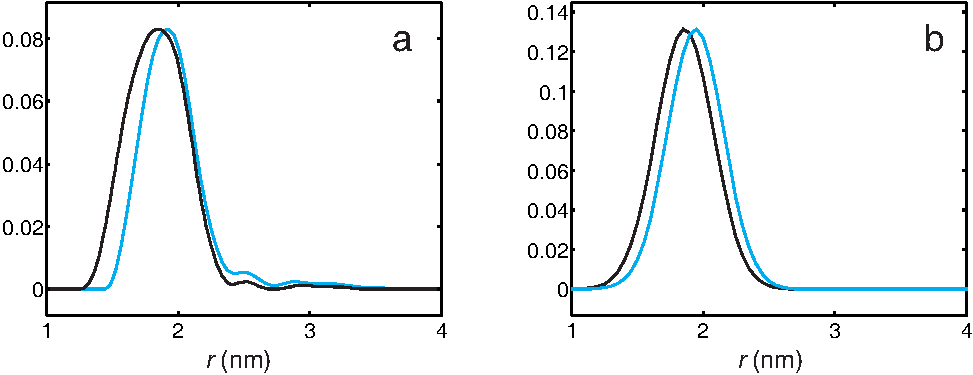
\includegraphics[width=1.0\textwidth]{fig7.pdf}
	\end{center}
	\caption{Excitation bandwidth correction. Blue distance distributions were obtained without, black ones with correction. a) Tikhonov regularization with optimum regularization parameter $\alpha=1$. b) Fit by a single Gaussian peak.}
	\label{fig:manfig7}
\end{figure}

However, simulations of the dipolar evolution function from a distance distribution, as they are required in model fits or at the end of Tikhonov regularization, can be performed with a pre-computed kernel for the expression given by eqn (\ref{eq:ideal_kernel}, while the kernel must be computed "on-the-fly" for the expression given by eqn (\ref{eq:real_kernel}. This is because the latter expression depends on an additional variable parameter $\Delta \omega$ and, furthermore, does not allow for scaling. In the former expression, a scaling of the $t$ axis by a factor $x$ can be compensated by scaling of the distance axis by a factor $x^{1/3}$. Without bandwidth correction, DeerAnalysis2018 uses fast computations with a pre-computed ideal kernel. Therefore, bandwidth correction considerably slows down simulations and model fits and is thus not selected as default behavior of the program. It can be activated by selecting the {\ttfamily Exci. bandwidth} checkbox in the {\ttfamily Dipolar evolution} panel.

The effect of excitation bandwidth correction is illustrated in Fig. \ref{fig:manfig7} for data set {\ttfamily deer\_bi\_oligo\_n8\_50K} from the {\ttfamily calibdepth} subdirectory. Data were cut off at 1504 ns to improve the background fit. Without correction (blue distributions) distances below 1.75 nm are strongly suppressed. With correction they are recovered. The r.m.s. deviation improves from 0.000320 without correction to 0.000286 with correction in Tikhonov regularization and from 0.000396 without correction to 0.000335 with correction for a Gaussian fit. An improvement in the r.m.s. value may not always be found. The mean distance obtained with Tikhonov regularization changes from 1.97 to 1.85 nm. For a slightly longer flexible biradical (data set {\ttfamily deer\_bi\_oligo\_n10\_50K}), the correction is somewhat smaller, as the mean distance changes from 2.07 to 1.98 nm (data not shown). Note also that the Gaussian fits do not account very nicely for the true shape of the distribution in this case.

\subsection{Ghost suppression}
\label{ghost_suppression}
If more than two spin labels are present in a nanoobject, sum and difference combinations appear in the DEER signal \cite{jeschke2009b}. This leads to ghost peaks in distance distributions that can be suppressed by power scaling of the form factor with an exponent $1/(N-1)$, where $N$ is the number of spins per nanoobject, for instance the number of protomers in a symmetric protein homooligomer \cite{vonHagens2013}. Such ghost suppression can be performed by activating the checkbox {\ttfamily ghost suppression} in the {\ttfamily Form factor} panel and inserting the number of spins in the edit field on the right of this checbox. It is advisable to perform data processing both with and without such suppression and to compare the distance distributions obtained. For detailed discussion of performance and limitations, see \cite{vonHagens2013}.


\subsection{Test data sets}
DeerAnalysis2018 has a subdirectory {\ttfamily simulated} with Matlab scripts for generating test data with artificial noise and artificial background. The directory also contains a number of such test data sets: Gaussian distributions, distributions with two Gaussian peaks, a boxcar distribution, and a sawtooth distribution. These data sets are intended for test and training purposes.

Test data sets are loaded by selecting the {\ttfamily ASCII} subpanel of the {\ttfamily Data sets} panel. The default column assignment (Time 1, Real 2, Imaginary 3) applies. These data sets can be processed in the same way as experimental data sets. In the {\ttfamily Distance distribution} plot of the main window and of the validation tool the distance distribution used for generating these data sets is displayed in cyan color.

Precomputed test data sets are a series of Gaussian distributions with fixed ratio of ten between mean distance and standard deviation, a boxbar from 2 to 4 nm, a sawtooth from 2 to 4 nm, Gaussian distributions at 3 and 4 nm with two-dimensional background, and a few distributions consisting of two Gaussian peaks. Further test data sets can be computed by using the Matlab scripts {\ttfamily create\_test\_data.m} (single Gaussian, 3D background), {\ttfamily create\_test\_data\_2D.m} (single Gaussian, 2D background), {\ttfamily create\_test\_data\_nb.m} (two Gaussians), {\ttfamily create\_test\_data\_special.m} (boxcar), {\ttfamily create\_test\_data\_special\_2.m} (sawtooth), and {\ttfamily create\_test\_data\_special\_3.m}.

\section{Error analysis (validation) of distance distributions}
\label{validation}
For an ill-posed problem the relation between noise in the input data and uncertainty of the output data is difficult to predict. Furthermore, background deconvolution is not exact for experimental data, which also introduces an error in the form factor. Often this error due to imperfect background correction even dominates the error in distance distribution.

While error propagation in Tikhonov regularization cannot be predicted analytically, there is an obvious numerical approach for such a prediction. Assume that the uncertainties of background correction can be modelled by variation of the starting time for the background fitting within certain bounds and of the dimensionality of the spatial distribution within certain bounds. Background correction can now be performed for a sufficiently large number $n_\mathrm{trials}$ of parameter sets within these bounds and the form factors obtained can be subjected to Tikhonov regularization. This provides $n_\mathrm{trials}$ distance distributions that can be statistically analyzed. Thus, a lower and upper limit, a mean value, and a standard deviation are obtained for each point in the distance distribution.

Alternatively, uncertainty of background parameters can be given in terms of lower and upper bounds for the density (proportional to concentration), the modulation depth, and the background dimensionality. This approach was followed until DeerAnalysis2010 and is still available for backward compatibility. This old approach does not consider that the uncertainties in the background parameters may be correlated. Thus it tends to overestimate the error. It is more advisable to vary the starting time for the background fit and, if necessary, background dimensionality.

Still, some combinations of dimensionality and starting time may result to poor fits of the form factor. A poor fit can be defined as a fit whose root mean square deviation from the experimental data exceeds the root mean square deviation (r.m.s.d.) of the best fit by a factor $L_\mathrm{prune}$ (prune level). DeerAnalysis2018 suggests a prune level of 1.15, but users can define this value according to their own experience. Parameter combinations that lead to fits with r.m.s.d. > \emph{prune level} $\cdot$ min(r.m.s.d.) are excluded from statistical analysis. 

The influence of noise on the distance distribution can be estimated in a similar way as the influence of uncertainties in background parameters. In this case noise is artificially enhanced by adding pseudorandom numbers so that the noise level is increased by a certain factor $L_\mathrm{noise}$. Errors are probably overestimated when taking $L_\mathrm{noise}=2$. A value $L_\mathrm{noise}=1.5$ is suggested. The tests for noise and background influence can be combined to obtain a total error estimate.

\begin{figure}[ht]
 	\begin{center}
  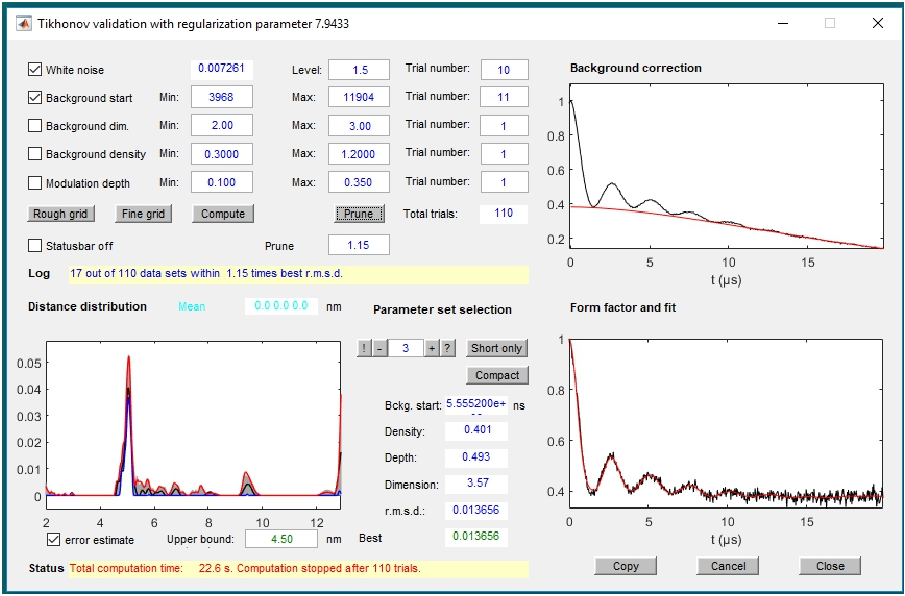
\includegraphics[width=1.0\textwidth]{fig10.pdf}
	\end{center}
	\caption{Screenshot of the validation window.}
	\label{fig:validation}
\end{figure}

The validation tool is started by clicking on the {\ttfamily Validation} button in the {\ttfamily Tikhonov regularization} subpanel of the {\ttfamily Data analysis} panel. This button is set inactive when a Tikhonov regularization has not yet been performed. Validation uses the regularization parameter that is selected in the main window when the button is clicked. This regularization parameter is displayed in the title line of the validation window (Figure \ref{fig:validation}) 

The user can now select what parameters have to be treated as uncertain (default: Background starting time), what lower and upper bounds are estimated for these parameters and how many values within these bounds should be tested. The trial values are distributed uniformly between the bounds. Each allowed value of each variable parameter is combined with each allowed value of each other parameter. One should be aware that this may lead to large numbers of trials and that for each trial a Tikhonov regularization has to be performed. Computation times may be substantial. The {\ttfamily Rough grid} and {\ttfamily Fine grid} buttons make suggestions for the bounds and number of trials that are based on the result of the background correction performed in the main window. These suggestions should only be used if there is no independent information on the bounds.

After starting the computation by clicking on the {\ttfamily Compute} button, a progress bar will appear as soon as the first Tikhonov regularization has been performed. At that point an estimate of the remaining computation time is displayed. If necessary the computation can be interrupted by closing the progress bar. For that the $\times$ button in the upper right corner of the progress bar has to be clicked. After the next Tikhonov regularization is completed, a window appears that allows for interrupt or continuation of the computation.

After all trials are computed the {\ttfamily Distance distribution} plot displays the distance distribution with the best r.m.s.d. as bold green line, grey error bars that indicate the full variation of the probability of a given distance over all trials, a lower error estimate corresponding to the mean value of the probability minus two times its standrad deviation, and an upper error estimate corresponding to the mean value plus two times the standard deviation (red dotted lines). The mean distance is indicated by a vertical cyan dotted line. For test data sets, the distance distribution used in simulating the data is displayed as a cyan solid line. By using the {\ttfamily -} and {\ttfamily +} buttons left and right from the data set number display, all computed distance distributions (and the corresponding background functions and fits iof the form factor) can be inspected in turn. The {\ttfamily Short only} button selects the data set with the smallest contribution of long distances. The {\ttfamily Compact} button selects the set with the most narrow distribution. The {\ttfamily ?} button selects the data set with largest r.m.s.d. of the fit from the experimental form factor and the {\ttfamily !} button the data set with the lowest r.m.s.d. 

Poor fits can now be excluded from statistical analysis by selecting the prune level and clicking on the {\ttfamily Prune} button. Note that this is irreversible. The excluded data sets are lost and can only be recovered by repeating the computation.

Separate Matlab figures of all plots (for copying, saving or printing) are obtained with the {\ttfamily Copy} button. The validation tool can be left either with the {\ttfamily Cancel} button, leaving the original state of the main window intact, or with the {\ttfamily Close} button, transferring the mean distance distribution and the error bounds to the main window. A report of the validation is stored automatically in the latter case.

After returning to the main window, the mean distance distribution from all trials is displayed. If the {\ttfamily error est.} option in the {\ttfamily Distance distribution} panel is selected, the lower and upper error bounds (two times standard deviation) are displayed as grey error bars.

\section{Post-processing}
\label{postprocess}
For many cases, one wants to quantify the distance distribution in terms of a few
numbers, i.e., mean distance and width of the whole distribution or of individual
peaks. For oligomers of membrane proteins and self-assembled supramolecular
systems, it may also be of interest to derive the number of spins within an
individual nanoobject. All these values can be obtained by post-processing.

\subsection{Moment analysis and peak picking}
Analysis of a number of simulated and experimental DEER data sets suggested
that the first moment (mean distance) and second moment (variance, square of
the standard deviation) of the distance distribution are stable parameters. In
other words, these values are only very slightly influenced by noise-induced artificial splittings in the distance distribution. This applies
in particular to the results of those techniques that incorporate the constraint
$P(r) > 0$ (Tikhonov regularization and model fitting). Moment analysis of the distance distribution in the range of interest (default: 1.5-8 nm) is therefore performed automatically. The mean distance ($\left\langle r \right\rangle$) and standard deviation (s(r)) are displayed in the {\ttfamily Distance analysis} panel. To exclude obvious artifacts
at the short or long end of the distance range (due to nuclear modulations or
errors in background correction), you may change the range for analysis using
the {\ttfamily +} and {\ttfamily -} buttons for the blue and magenta cursor in the {\ttfamily Distance distribution} panel or direct input into the corresponding edit fields. This option can also be used for extending the distance range if very long distances have been measured or for selecting only a single peak in a multimodal distance distribution and determining its mean distance and width.  When the {\ttfamily Expand} checkbox is selected, the distance distribution is displayed only between the cursors. 

\subsection{Checking for the relevance of small peaks}
With Tikhonov regularization, one sometimes observes small peaks in the distance distribution that may be related to noise, to errors in background correction, or to genuine small contributions to the distance distribution. It is instructive to check the contribution of such peaks to the simulated dipolar evolution function or dipolar spectrum. To suppress such peaks, move the blue and magenta cursors so that they include them (see Fig. \ref{fig:manfig8}) and click on the green {\ttfamily Suppress} button. The distance distribution without these peaks is shown as a green curve and the corresponding fit of the experimental data is displayed in the {\ttfamily Dipolar evolution} plot also as a green curve. In the case illustrated in Fig. \ref{fig:manfig8}, the small peaks are obviously artifacts. The original (red) fit has a slightly better r.m.s. value, but is not perfect (see first minimum of the oscillation). The green fit is better at the first minimum but worse at the second maximum. In this case, the small peaks should thus be disregarded in interpretation.

\begin{figure}[ht]
 	\begin{center}
  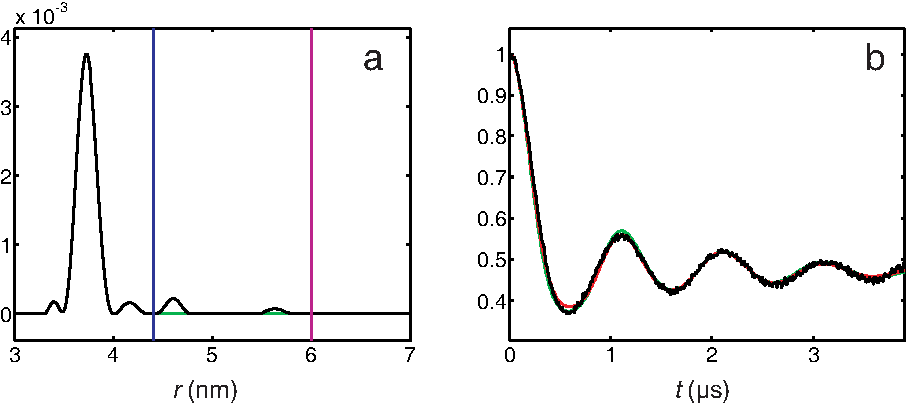
\includegraphics[width=1.0\textwidth]{fig8.pdf}
	\end{center}
	\caption{Suppressing small peaks in data set {\ttfamily deer\_bi\_36\_50K} from the {\ttfamily calibdepth} subdirectory. a) Distance distribution obtained by Tikhonov regularization (black) and after suppressing the peaks between the blue and magenta cursor by clicking on the green {\ttfamily Suppress} button (green). b) Experimental duipolar evolution function (black), fit by Tikhonov regularization (red), and fit after suppressing the two small peaks between the blue and magenta cursor.}
	\label{fig:manfig8}
\end{figure}


\subsection{Number of coupled spins}
\label{numspins}
The number of spins within a nanoobject can be derived from the (calibrated)
modulation depth if decay due to spins in other nanoobjects can be neglected,
as was shown early on by the Novosibirsk group \cite{milov1984}. The same applies for
the modulation depth in the dipolar evolution function after appropriate correction
of the background decay \cite{jeschke2004a}. The total modulation depth is given by
\begin{equation}
	\Delta = 1 - \exp \left[ \lambda \left( \left\langle n \right\rangle - 1 \right) \right] \; ,
\end{equation}
where $\left\langle n \right\rangle$ is the average number of spins in the observed nanoobjects.
 
To use this information, DeerAnalysis2018
therefore retains information on the modulation depth in the dipolar evolution function. Quantification requires knowledge of the modulation depth parameter $\lambda$, which depends strongly on the excitation position, length, and flip angle of the pump pulse and weakly on line broadening
in the nitroxide spectrum and shape of the resonator mode. Reliable
quantification therefore requires a calibration with known samples and proper
adjustment of the flip angle of the pump pulse (see Section \ref{experimental}). Spectra from our own
series of calibration samples (six biradicals and one triradical) are provided in
the folder calibdepth. They correspond to 12 ns $\pi$ pump pulses irradiated at the
maximum of the nitroxide spectrum (see Fig. \ref{fig:manfig2}) using a Bruker 3mm split-ring
resonator. Note that not all example spectra in other folders were measured
under the same conditions. To calibrate modulation depths for your own applications,
you should measure at least one genuine biradical with close to 100\%
degree of spin-labeling under your measurement conditions. Analyse the data for this biradical, preferably with Tikhonov regularization and change the number of spins in the corresponding edit field of the {\ttfamily Distance analyis} panel to 2. The number is then displayed in green instead of red color. If another data set, measured under the same conditions, is loaded and processed, the displayed number of spins should correspond to the true average number $\left\langle n \right\rangle$ of spins in the nanoobject.

Note that this calibration is lost on restarting DeerAnalysis and that it is unreliable when using excitation bandwidth correction. Also consult Section \ref{localconc}.

\subsection{Comparing data sets (dual display)}
\label{dual_display}
To compare two data sets of the same sample or of similar samples first load one of the data sets and process it as usual. To keep the same processing parameters for the second data set, you may then want to uncheck the {\ttfamily Reset} checkbox below the {\ttfamily Load} button in the {\ttfamily Data sets} panel. After loading the second data set, its file name is shown in line {\ttfamily A:} of the {\ttfamily Data sets} panel. This is the active data set. The file name of the previous data set is shown in line {\ttfamily B:}. The original data and processing results can now be compared by selecting the {\ttfamily Dual display} checkbox in the {\ttfamily Original data} panel. Traces corresponding to the previous data set are now shown in blue in all plots. In the {\ttfamily Dipolar evolution} plot, only experimental data, but no fits are shown for the previous data set.

\begin{figure}[ht]
 	\begin{center}
  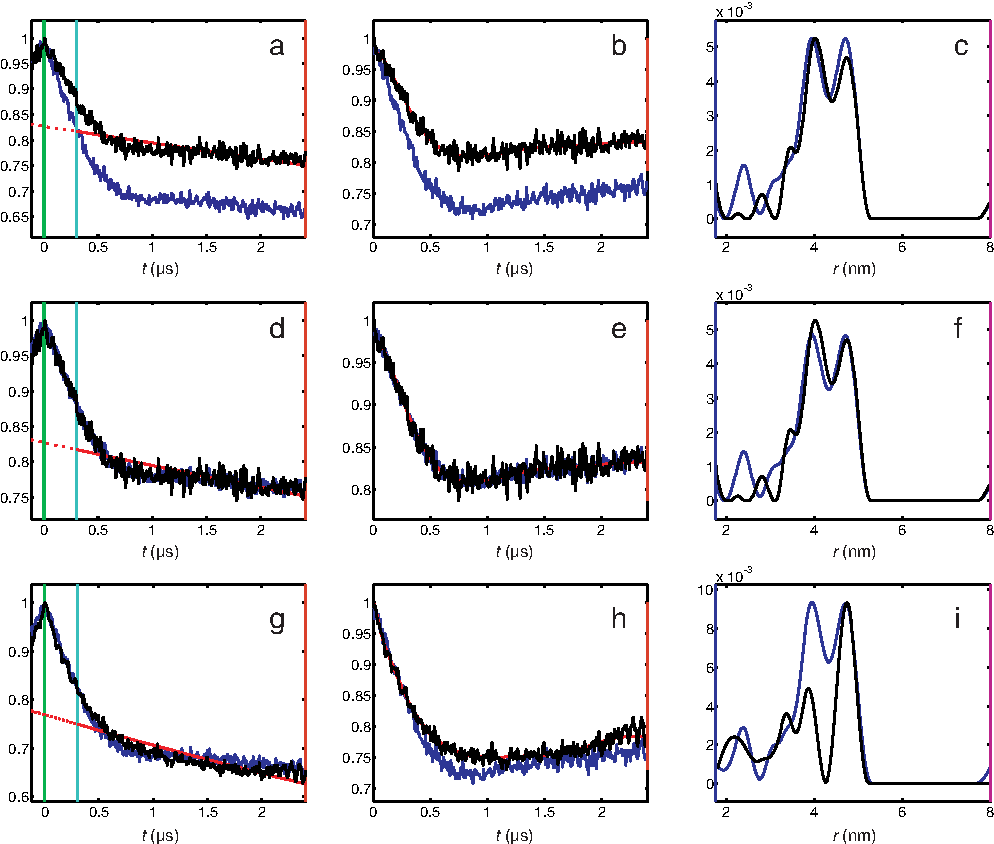
\includegraphics[width=0.9\textwidth]{fig9.pdf}
	\end{center}
	\caption{Dual display for comparison of two data sets. All data sets are from the subdirectory {\ttfamily examples$\backslash$series}. Left column: Original data. Middle column: Dipolar evolution functions after background correction. Right column: Distance distributions. a-c) Comparison of data sets {\ttfamily series2} (active set A, black traces) and {\ttfamily series1} (set B) without modulation depth scaling. d-f) Comparison of data sets {\ttfamily series2} (active set A, black traces) and {\ttfamily series1} (set B) with modulation depth scaling. g-i) Comparison of data sets {\ttfamily series8} (active set A, black traces) and {\ttfamily series1} (set B) with modulation depth scaling. }
	\label{fig:manfig9}
\end{figure}

If the two data sets differ considerably in their modulation depth, but have similar distance distribution, the samples may just differ in the extent of spin labelling or the measurement conditions (flip angles, resonator, pulse lengths) may have been slightly different. To check for this, use modulation depth scaling \cite{jeschke2004a} by selecting the {\ttfamily mod. depth scaling} checkbox in the {\ttfamily Original data} panel. Differences in the distance distribution are noise-related if the original data are not significantly different after such modulation depth scaling.

\section{Output}
\subsection{Saving data}
\label{output}
Unlike its early predecessor version, DeerAnalysis2018 does not automatically save results, except as an option during processing series of data sets (see Section \ref{series}). On attempt to close the program after time-consuming fits (Tikhonov regularization, model fits) without saving results, the user is reminded. The whole set of data including background correction, experimental and fitted dipolar evolution function and spectrum, distance distribution, processing parameters, results of moment analysis and fitted parameters and L curve (if available) are saved together with the same basis file name, but into different ASCII files. 

After clicking on the {\ttfamily Save} button, the user is asked for the file name. The last extension and, if present, a suffix {\ttfamily \_res} are removed to derive the basis name {\ttfamily \emph{basname}} (this is useful for overwriting old results by selecting their name in the diplayed file list). The following files are then saved:

\begin{tabular}{ll}
\noalign{\smallskip}
$\bullet$ & {\ttfamily \emph{basname}\_res.txt} \\
& a summary of the program settings and the results \\
$\bullet$ & {\ttfamily \emph{basname}\_bckg.dat} \\
& the phase-corrected original data and background fit \\
& $1^{st}$ column: time axis (in $\mu$s), \\
& $2^{nd}$ column: real part of original data, \\
& $3^{rd}$ column: background fit \\
& $4^{th}$ column: imaginary part of original data (if present) \\
$\bullet$ & {\ttfamily \emph{basname}\_fit.dat} \\
& the dipolar evolution function and its fit \\
& $1^{st}$ column: time axis (in $\mu$s), \\
& $2^{nd}$ column: dipolar evolution function after background correction, \\
& $3^{rd}$ column: fit of the dipolar evolution function \\
$\bullet$ & {\ttfamily \emph{basname}\_spc.dat} \\
& the dipolar spectrum and its fit \\
& $1^{st}$ column: frequency axis (in MHz), \\
& $2^{nd}$ column: experimental dipolar spectrum, \\
& $3^{rd}$ column: fit of the dipolar spectrum \\
$\bullet$ & {\ttfamily \emph{basname}\_distr.dat} \\
& the distance distribution \\
& $1^{st}$ column: distance axis (in nm), \\
& $2^{nd}$ column: distance distribution $P(r)$ \\
$\bullet$ & {\ttfamily \emph{basname}\_Lcurve.dat} \\
& the L curve of Tikhonov regularization (only if computed) \\
& $1^{st}$ column: log($\rho$), \\
& $2^{nd}$ column: log($\eta$), \\
& $3^{rd}$ column: corresponding regularization parameters $\alpha$ \\
\end{tabular}

The results file {\ttfamily \emph{basname}\_res.txt} protocols all relevant program settings,
the mean distance, width of the distance distribution, and third moment,
and for Tikhonov regularization, the regularization parameter. For model fits, the values of all fit parameters are also saved here.

\subsection{Copying or printing individual plots}
The three current plots of DeerAnalysis2018 can be copied into individual Matlab figures by clicking on the {\ttfamily Copy} button in the {\ttfamily Data sets} panel. Using the figure menu, the plots can then be rescaled, edited, annotated, printed, exported as different graphics formats or copied into the Windows clipboard (item {\ttfamily Copy figure} in the {\ttfamily Edit} menu). Matlab has a good help system that explains these possibilities.  

\section{Processing a series of similar data sets}
\label{series}

A global analysis of several data sets is useful when measurements on the same sample have been reproduced or when samples have been prepared under slightly different conditions and one wants to check whether structural changes have occurred (see also Section \ref{dual_display}). The first case requires computation of an average distance distribution that takes into account the signal-to-noise ratio of the individual data sets. In the second case the comparison should be performed for modulation-depth normalized primary data rather than for distance distributions as it is difficult to estimate what degree of change in the distance distribution is significant \cite{jeschke2004a}. For both tasks a text file {\ttfamily \emph{listname}.txt} has to be prepared that contains a list of filenames (without extension) of all the data sets that are to be processed together (for an example, see the file {\ttfamily series.txt} in the subdirectory {\ttfamily example$\backslash$series}).

List processing starts with analysis of a pilot data set, which should ideally be the data set with the best signal-to-noise ratio. This data set with best signal-to-noise ratio should also be the first set in the list, as the first data set is used as a reference for modulation depth scaling. After loading the pilot data set it is processed as usual. Series processing is then initiated by the {\ttfamily Series} button in the {\ttfamily Data sets} panel. Progress is reported in the {\ttfamily Status} panel and line {\ttfamily A:} of the {\ttfamily Data set} panel. Plots are also updated (with a slight delay) during series processing. The program will return after the last data set has been processed. This data set is now the active data set.

The average distance distribution and average dipolar evolution function after series processing as well as average results of moment analysis are not displayed on screen, but are saved automatically. These files have the following formats:

\begin{tabular}{ll}
\noalign{\smallskip}
$\bullet$ & {\ttfamily \emph{listname}\_res.txt} \\
& a summary of the program settings and the results for the average \\
& of all data sets \\
$\bullet$ & {\ttfamily \emph{listname}\_mean.dat} \\
& the mean dipolar evolution function \\
& $1^{st}$ column: time axis (in $\mu$s), \\
& $2^{nd}$ column: mean dipolar evolution function after background \\
& correction, \\
$\bullet$ & {\ttfamily \emph{listname}\_cmp.dat} \\
& modulation-depth normalized primary data (without background \\
& correction) \\
& $1^{st}$ column: time axis (in $\mu$s), \\
& $n$ remaining columns: primary data (real part) for data sets $1\cdots n$, \\
$\bullet$ & {\ttfamily \emph{listname}\_diff.dat} \\
& $n \times n$ matrix quantifying the difference between data sets \\
& large values in element $(k,j)$ indicate that data sets $k$ and $j$ differ \\
& significantly \\
\end{tabular}

Primary data sets and distance distributions are averaged with a weighting factor that is inversely proportional to the mean square deviation of the fit of the dipolar evolution function. This corresponds to a maximum likelihood estimate of the average.

By default results for the individual data sets are not automatically saved. Automatic saving can be initiated by selecting the {\ttfamily Autosave} checkbox below the {\ttfamily Series} button. Note that even with this checkbox selected, automatic saving takes place only during series processing, not when processing individual data sets via the {\ttfamily Load} button.

\section{Hints for Data Acquisition}
\label{experimental}

Conversion of a dipolar evolution function as measured by a magnetic resonance experiment to a distance distribution is an ill-posed mathematical problem \cite{jeschke2001}. This means that even small deviations from the theoretical function (noise, phase problems, an intensity offset) can cause significant distortions in the distance distribution. Thus, it is of utmost importance to acquire experimental data with the {\em best} quality possible within a reasonable measurement time.

The choice of a number of experimental parameters has been discussed earlier \cite{jeschke2002}. From our own experience we suggest to perform measurements in the following way. A temperature of 80 K is a good compromise for most samples, but sensitivity is often somewhat better at 50 K. For critical samples such as membrane proteins, cooling to 50 K is often worth the effort. Unless the sample really has a strong signal, one should plan for measuring two samples in 24 hours, one during the day and one over night. Spectrometers tend to be stable enough over a period of several hours and the quality of the distance distribution tends to be limited by the signal-to-noise ratio except for synthetic model compounds with very narrow distance distributions. The observer and pump frequencies should be stable within 1 MHz during the measurement time, and this should be checked. It is good practice to acquire data with quadrature detection and to adjust the detector phase properly at the beginning. That way instability of the spectrometer can be recognized by the appearance of a significant imaginary part of the signal. Note that a small phase drift (corrections up to 20$^{\circ}$ for a measurement extending over several hours) is no cause for alarm.

For four-pulse DEER on pairs of nitroxides at X-band frequencies we suggest that the pump pulse has a length of 12 ns. This can be achieved with a Bruker 3-mm-split-ring resonator. We also suggest that all the observer pulses have the same length of 32 ns. These conditions cannot be met at all spectrometers and with all probeheads. Using a length of 32 ns for all pulses, or a length of 16 ns for the $\pi$/2 pulses and a length of 32 ns for the $\pi$ pulses also provides good results. If your pump $\pi$ pulse has the same length as the $\pi$ observer pulses, you may want to set the observer frequency to the center of the resonator mode and the pump frequency into the flank. Note however, that the opposite setting as suggested by Fig. \ref{fig:manfig2} allows for a shorter pump pulse and hence larger modulation depth.

The power of the pump pulse should be adjusted for optimum flip angle (optimum echo inversion) using an inversion recovery sequence $\pi_{\mathrm{pump}}-T-\pi/2_\mathrm{obs}-\tau-\pi_{\mathrm{obs}}-\tau-echo$ . This has to be done with coinciding pump and observer frequency at the position in the microwave mode where the pump pulse is applied. After this step the pump frequency should not be changed anymore. If this procedure is not followed, modulation depths are ill-defined and should not be compared between samples. The step is also an absolute requirement if concentrations are to be determined. We suggest that the pump pulse is applied at the maximum of the nitroxide spectrum, which maximizes modulation depth. This minimizes artifacts due to nuclear modulations, phase noise, and spectrometer imperfections.

The observer pulses are then applied at the low-field local maximum which corresponds to increasing the observer frequency (spectrometer frequency) by approximately 65 MHz. You may measure the field difference $\Delta B_{0}$ between the two maxima and multiply it by 2.8 to obtain the exact frequency difference for your particular nitroxide. A phase cycle $(+x)-(-x)$ should be applied to the first observer pulse to eliminate offsets in the detector channels. If this phase cycling is omitted, any phase correction of the primary data will not be exact and hence background correction by program DeerAnalysis2018 will not be exact. Furthermore, modulation depth information is not reliable. In principle, the problems could be solved by introducing the offset as an additional parameter in background correction, but we strongly discourage such an approach, as it complicates separation of the dipolar evolution function from the background which may be difficult anyway for long distances.

For the interpulse delays in the four-pulse DEER experiment $\pi$/2($\nu_{\mathrm{obs}}$)-$\tau_{1}$-$\pi$($\nu_{\mathrm{obs}}$)-$t'$-$\pi$($\nu_{\mathrm{pump}}$)-($\tau_{1}$+$\tau_{2}$-$t'$)-$\pi$($\nu_{\mathrm{obs}}$)-$\tau_{2}$-{\em echo} we suggest $\tau_{1} = 200$ ns for protonated solvents/matrices and $\tau_{1} = 400$ ns for deuterated solvents/matrices (at X band). To suppress proton modulations it is advantageous to perform the experiment at eight different values of $\tau_{1}$ spaced by 8 ns and starting with the values given above. The signals of the eight experiments are added. In variable-time DEER \cite{jeschke2004b} we suggest initial values $\tau_{2,0}= 300$ ns for protonated and $\tau_{2,0}= 500$ ns for deuterated samples. In constant-time DEER, $\tau_{2} = 800$ ns is usually convenient for setup (adjustment of the detector phase). For the actual measurement, the choice of $\tau_{2}$ depends on transverse relaxation, signal strength, and on the longest distances that have to be measured. It is difficult to give general suggestions, but the problem has been discussed in some detail in Ref. \cite{jeschke2004b}.

The integration gate should match the width of the observer echo, which is similar to the width of the longest observer pulses. The gate should be centered at the echo maximum. If you can save data in Xepr (Elexsys) format, DeerAnalysis 2004 can directly import binary data. For ESP 380 data we suggest importing them into WIN-EPR and saving them in the {\em binary} WIN-EPR format (this step converts the coding of binary float numbers to a format legible by MATLAB). If you use another data acquisition system, you should save your data in an ASCII representation. 

\section*{Acknowledgments}
\label{acknowledge}
We thank Freiburger Materialforschungszentrum for the FTIKREG Tikhonov regularization code by J. Weese, G. Milhauser for helping with implementation of a Mac version, and M. Spitzbarth, S. Domingo K\"ohler, and M. Drescher for implementing the Rice distribution model.    
 
% The Appendices part is started with the command \appendix;
% appendix sections are then done as normal sections
% \appendix

% \section{}
% \label{}

\begin{thebibliography}{00}

% \bibitem{label}
% Text of bibliographic item

% notes:
% \bibitem{label} \note

% subbibitems:
% \begin{subbibitems}{label}
% \bibitem{label1}
% \bibitem{label2}
% If there is a note, it should come last:
% \bibitem{label3} \note
% \end{subbibitems}

\bibitem{jeschke2009}
G. Jeschke, M. Sajid, M. Schulte, A. Godt.
{\em Phys. Chem. Chem. Phys.} {\bf 11} (2009) 6580--6591.

\bibitem{jeschke2006}
G. Jeschke, V. Chechik, P. Ionita, A. Godt, H. Zimmermann, J. Banham, C. R. Timmel, D. Hilger, H. Jung.
{\em Appl. Magn. Reson.} {\bf 30} (2006) 473--498.

\bibitem{dalmas2012}
O. Dalmas, H. C. Hyde, R. E. Hulse, E. Perozo. 
{\em J. Am. Chem. Soc.} {\bf 134} (2012) 16360-16369.


\bibitem{pannier2000}
M. Pannier, S. Veit, A. Godt, G. Jeschke, H. W. Spiess,
{\em J. Magn. Reson.} {\bf 142} (2000) 331--340.

\bibitem{jeschke2004b}
G. Jeschke, A. Bender, H. Paulsen, H. Zimmermann, A. Godt,
{\em J. Magn. Reson.} {\bf 169} (2004) 1--12.

\bibitem{jeschke2004a}
G. Jeschke, G. Panek, A. Godt, A. Bender, H. Paulsen,
{\em Appl. Magn. Reson.} {\bf 26} (2004) 223-244.

\bibitem{jeschke2001}
G. Jeschke, A. Koch, U. Jonas, A. Godt,
{\em J. Magn. Reson.} {\bf 155} (2001) 72--82.

\bibitem{borbat1999}
P.P. Borbat, J.H. Freed,
{\em Chem. Phys. Lett.} {\bf 313} (1999) 145--154.

\bibitem{jeschke2003b}
G. Jeschke, A. Godt,
{\em ChemPhysChem} {\bf 4} (2003) 1328--1334.

\bibitem{sifter}
G. Jeschke, M. Pannier, A. Godt, H. W. Spiess,
{\em Chem. Phys. Lett.} {\bf 331} (2000) 243--252.

\bibitem{hinderbe2004}
D. Hinderberger, H. W. Spiess, G. Jeschke,
{\em J. Phys. Chem.} {\bf 108} (2004) 3698--3704.

\bibitem{godt2006}
A. Godt, M. Schulte, H. Zimmermann, G. Jeschke,
{\em Angew. Chem. Int. Ed.} {\bf 45} (2006) 7560--7564.

\bibitem{vonHagens2013}
T. von Hagens, Y. Polyhach, M. Sajid, A. Godt, G. Jeschke.
{\em Phys. Chem. Chem. Phys.} {\bf 15} (2013) 5854--5866.

\bibitem{koehler2011}
S. Domingo K\"ohler, M. Spitzbarth, K. Diederichs, T. E. Exner, M. Drescher,
{\em J. Magn. Reson.}, {\bf 208} (2011) 167--170.

\bibitem{jeschke2002}
G. Jeschke,
{\em ChemPhysChem} {\bf 3} (2002) 927--932.

\bibitem{freed2005}
Y. W. Chiang, P. P. Borbat, J. H. Freed,
{\em J. Magn. Reson.} {\bf 172} (2005) 279--295.

\bibitem{maryasov2000}
A. G. Maryasov, Y. D. Tsvetkov, 
{\em Appl. Magn. Reson.} {\bf 18} (2000) 583--605.

\bibitem{milov2004}
A. D. Milov, B. D. Naumov, Y. D. Tsvetkov,
{\em Appl. Magn. Reson.} {\bf 26} (2004) 587--599.

\bibitem{tikhonov}
A. N. Tikhonov, V. Y. Arsenin, 
{\em Solutions of Ill-Posed Problems} (Wiley, New York, 1977).

\bibitem{honerkamp1990}
J. Honerkamp, J. Weese,
{\em Cont. Mech. Therm.} {\bf 2} (1990) 17.

\bibitem{weese1992}
J. Weese,
{\em Comput. Phys. Commun.} {\bf 69} (1992) 99--111 (1992).

\bibitem{milov1984}
A. D. Milov, A. B. Ponomarev, Y. D. Tsvetkov,
{\em Chem. Phys. Lett.} {\bf 110} (1984) 67--72.

\bibitem{jeschke2009b}
G. Jeschke, M. Sajid, M. Schulte, A. Godt,
{\em Phys. Chem. Chem. Phys.} {\bf 11} (2009) 6580--6591.

\bibitem{edwards2018}
T.~H.~Edwards, S.~Stoll
{\em J.~Magn.~Reson.} {\bf 288} (2018) 58-68.

\end{thebibliography}

\end{document}

